\documentclass[nohyper,justified,marginals=raggedright]{tufte-book}\usepackage[]{graphicx}\usepackage[]{color}
%% maxwidth is the original width if it is less than linewidth
%% otherwise use linewidth (to make sure the graphics do not exceed the margin)
\makeatletter
\def\maxwidth{ %
  \ifdim\Gin@nat@width>\linewidth
    \linewidth
  \else
    \Gin@nat@width
  \fi
}
\makeatother

\definecolor{fgcolor}{rgb}{0.345, 0.345, 0.345}
\newcommand{\hlnum}[1]{\textcolor[rgb]{0.686,0.059,0.569}{#1}}%
\newcommand{\hlstr}[1]{\textcolor[rgb]{0.192,0.494,0.8}{#1}}%
\newcommand{\hlcom}[1]{\textcolor[rgb]{0.678,0.584,0.686}{\textit{#1}}}%
\newcommand{\hlopt}[1]{\textcolor[rgb]{0,0,0}{#1}}%
\newcommand{\hlstd}[1]{\textcolor[rgb]{0.345,0.345,0.345}{#1}}%
\newcommand{\hlkwa}[1]{\textcolor[rgb]{0.161,0.373,0.58}{\textbf{#1}}}%
\newcommand{\hlkwb}[1]{\textcolor[rgb]{0.69,0.353,0.396}{#1}}%
\newcommand{\hlkwc}[1]{\textcolor[rgb]{0.333,0.667,0.333}{#1}}%
\newcommand{\hlkwd}[1]{\textcolor[rgb]{0.737,0.353,0.396}{\textbf{#1}}}%

\usepackage{framed}
\makeatletter
\newenvironment{kframe}{%
 \def\at@end@of@kframe{}%
 \ifinner\ifhmode%
  \def\at@end@of@kframe{\end{minipage}}%
  \begin{minipage}{\columnwidth}%
 \fi\fi%
 \def\FrameCommand##1{\hskip\@totalleftmargin \hskip-\fboxsep
 \colorbox{shadecolor}{##1}\hskip-\fboxsep
     % There is no \\@totalrightmargin, so:
     \hskip-\linewidth \hskip-\@totalleftmargin \hskip\columnwidth}%
 \MakeFramed {\advance\hsize-\width
   \@totalleftmargin\z@ \linewidth\hsize
   \@setminipage}}%
 {\par\unskip\endMakeFramed%
 \at@end@of@kframe}
\makeatother

\definecolor{shadecolor}{rgb}{.97, .97, .97}
\definecolor{messagecolor}{rgb}{0, 0, 0}
\definecolor{warningcolor}{rgb}{1, 0, 1}
\definecolor{errorcolor}{rgb}{1, 0, 0}
\newenvironment{knitrout}{}{} % an empty environment to be redefined in TeX

\usepackage{alltt}

% \IfFileExists{bergamo.sty}{\usepackage[osf]{bergamo}}{}% Bembo
% \IfFileExists{chantill.sty}{\usepackage{chantill}}{}% Gill Sans
% \usepackage{lmodern}

\usepackage[T1]{fontenc}
\usepackage{xcolor}
\usepackage{colortbl}
\usepackage{fancyhdr}
\usepackage{xfrac}
\setlength{\headheight}{15pt}
\pagestyle{fancy}
\renewcommand{\chaptermark}[1]{ \markboth{#1}{} }
\renewcommand{\sectionmark}[1]{ \markright{#1}{} }

\fancyhf{}
\fancyhead[LE,RO]{\thepage}
\fancyhead[RE]{\textit{ \nouppercase{\leftmark}} }
\fancyhead[LO]{\textit{ \nouppercase{\rightmark}} }

\fancypagestyle{plain}{ %
  \fancyhf{} % remove everything
  \renewcommand{\headrulewidth}{0pt} % remove lines as well
  \renewcommand{\footrulewidth}{0pt}
}
\renewcommand{\headrulewidth}{\iffloatpage{0pt}{0.4pt}}
\clearpage{\pagestyle{empty}\cleardoublepage}

\usepackage{subfig}

\usepackage{url}
\usepackage[unicode=true,
 pdfusetitle,
 bookmarks=true, bookmarksnumbered=true,bookmarksopen=true, bookmarksopenlevel=2,
 breaklinks=true,
 pdfborder={0 0 1},
 backref=false,
 colorlinks=true,linkcolor=blue,citecolor=blue,urlcolor=blue,
 pdftitle={Practical Psychometrics},
 pdfsubject={A Psychological Assessment Toolkit},
 pdfkeywords={psychometrics,psychological assessment},
 pdfcreator=pdflatex]
 {hyperref}
\hypersetup{
 pdfstartview=FitH}
% \usepackage{breakurl}
\usepackage{amsmath}
\usepackage{amsfonts}
\usepackage{amssymb}
\usepackage{array}
\usepackage{mathtools}
% \usepackage[natbibapa]{apacite}
\usepackage{natbib}
\usepackage{tikz}
\usetikzlibrary{positioning}
\usetikzlibrary{decorations.pathreplacing}
\usetikzlibrary{arrows,shapes,backgrounds, shadows}
\usetikzlibrary{calc}
\tikzset{
  dot hidden/.style={},
  line hidden/.style={},
  dot colour/.style={dot hidden/.append style={color=#1}},
  dot colour/.default=black,
  line colour/.style={line hidden/.append style={color=#1}},
  line colour/.default=black
}

\usepackage{xparse}
\NewDocumentCommand{\drawdie}{O{}m}{
\begin{tikzpicture}[x=1em,y=1em,radius=0.1,#1]
  \draw[rounded corners=2,line hidden] (0,0) rectangle (1,1);
  \ifodd#2
    \fill[dot hidden] (0.5,0.5) circle;
  \fi
  \ifnum#2>1
    \fill[dot hidden] (0.25,0.25) circle;
    \fill[dot hidden] (0.75,0.75) circle;
   \ifnum#2>3
     \fill[dot hidden] (0.25,0.75) circle;
     \fill[dot hidden] (0.75,0.25) circle;
    \ifnum#2>5
      \fill[dot hidden] (0.75,0.5) circle;
      \fill[dot hidden] (0.25,0.5) circle;
     \ifnum#2>7
       \fill[dot hidden] (0.5,0.75) circle;
       \fill[dot hidden] (0.5,0.25) circle;
      \fi
    \fi
  \fi
\fi
\end{tikzpicture}
}  
\makeatletter

%%%%%%%%%%%%%%%%%%%%%%%%%%%%%% LyX specific LaTeX commands.

\title{Practical Psychometrics: A Psychological Assessment Toolkit}
\publisher{W. Joel Schneider}
% \publisher{Where You're From}
%%%%%%%%%%%%%%%%%%%%%%%%%%%%%% User specified LaTeX commands.
\renewcommand{\textfraction}{0.05}
\renewcommand{\topfraction}{0.8}
\renewcommand{\bottomfraction}{0.8}
\renewcommand{\floatpagefraction}{0.75}


\usepackage[buttonsize=1em]{animate}


\makeatother

\def\Rho{P}
\definecolor[named]{royalblue}{rgb}{0.26,0.43,0.93}
\definecolor[named]{firebrick}{RGB}{205,38,38}
\definecolor[named]{xBlue}{RGB}{0,0,255}
\definecolor[named]{xGreen}{RGB}{0,128,0}
\definecolor[named]{xPurple}{RGB}{153,0,204}
% \setsidenotefont{\color{royalblue!70}}
% \setcaptionfont{hfont commandsi}
\setmarginnotefont{\color{royalblue}}
\setcitationfont{\color{royalblue}}
\setlength\marginparpush{6mm}
% \let\oldmarginpar\marginpar
% \renewcommand\marginpar[1]{\-\oldmarginpar[\color{blue} #1]%
% {\color{blue} #1}}
\newcommand{\defword}[1]{\textbf{#1}} 
\newcommand{\citeapos}[1]{\citeauthor{#1}'s (\citeyear{#1})}

% Redefine boldsymbol
\newcommand{\bs}[1]{\boldsymbol{#1}}

\newenvironment{conditions}
  {\par\vspace{\abovedisplayskip}\noindent\begin{tabular}{>{$}c<{$} @{${}={}$} l}}
  {\end{tabular}\par\vspace{\belowdisplayskip}}
\usepackage{tabularx}
\newenvironment{conditions*}
{\par\vspace{\abovedisplayskip}\noindent
 \tabularx{\columnwidth}{>{$}c<{$} @{${}={}$} >{\raggedright\arraybackslash}X}}
{\endtabularx\par\vspace{\belowdisplayskip}}
\IfFileExists{upquote.sty}{\usepackage{upquote}}{}
\begin{document}


% \frontmatter
% \maketitle
\setcounter{secnumdepth}{1}
\setcounter{tocdepth}{1}
% \tableofcontents

% !Rnw root = Test.Rnw
\chapter{Notation}
Random variables are capital letters such as $X$ and $Y$.\\
A particular value of $X$ is $x$.\\
Vectors are bold lowercase symbols (e.g., $\boldsymbol{a}$, $\boldsymbol{\theta}$).\\
Matrices are bold uppercase symbols (e.g., $\boldsymbol{A}$, $\boldsymbol{\Theta}$).\\

Unfortunately, if vectors are lowercase and random variables are uppercase, my notation comes in conflict when discussing a vector of random variables (i.e., the variables as theoretical entities, not their particular scores). Such a vector will be a bold uppercase letter, (e.g., $\boldsymbol{X}$). A vector of particular scores from the variables in $\boldsymbol{X}$ will be shown as $\boldsymbol{x}$.

\begin{conditions*}
\phantomsection \label{note:R}\mathbb{R} & The set of all real numbers\\
\phantomsection \label{note:Z}\mathbb{Z} & The set of all integers\\
\phantomsection \label{note:N0}\mathbb{N}_0 & The set of all non-negative integers: $\{ 0,1,2,...\}$\\
\phantomsection \label{note:N1}\mathbb{N}_1 & The set of all positive integers: $\{ 1,2,3,...\}$\\
\phantomsection \label{note:Interval}\lbrack a,b\rbrack & The set of real numbers in the interval between $a$ and $b$\\
\phantomsection \label{note:In}\in & Is a member of\\
\phantomsection \label{note:binomial}\binom{n}{k} & The \emph{binomial coefficient}. It is just a shortcut notation for $\binom{n}{k}=\frac{n!}{k!\left(n-k\right)!}$. Read aloud, $\binom{n}{k}$ is ``$n$ choose $k$'' or the number of combinations that $n$ things have when taken $k$ at a time.\\
f_X(x;\boldsymbol{\theta}) & The probability density function or probability mass function of $X$ with parameters $\boldsymbol{\theta}$\\
F_X(x;\boldsymbol{\theta}) & The cumulative distribution function of $X$ with parameters $\boldsymbol{\theta}$\\
E(X) & The expected value of $X$\\
\mu_X, m_X & The population and sample mean of $X$\\
\sigma_X, s_X & The population and sample standard deviation of $X$\\
\sigma_X^2, s_X^2 & The population and sample variance of $X$\\
\gamma_1, g_1 & The population and sample skewness\\
\gamma_2, g_2 & The population and sample kurtosis\\
\boldsymbol{R_X} & The correlation matrix of the variables in vector $\boldsymbol{X}$\\
\boldsymbol{R_X} & The correlation matrix of the variables in vector $\boldsymbol{X}$\\
\bs{A'} & The transpose of matrix $\bs{A}$\\
\bs{A}^{-1} & The inverse of matrix $\bs{A}$\\
\mathtt{diag}(\bs{A}) & The column vector formed from the diagonal of matrix $\bs{A}$\\
\mathtt{diag}(\bs{a}) & The diagonal matrix formed from column vector $\bs{a}$\\
\bs{1} & A column vector of ones. Its length can be inferred by context.\\
\bs{I} & An identity matrix. Its dimensions can be inferred by context.\\
\end{conditions*}


% !Rnw root = Test.Rnw
\chapter{Introduction}
Although great painters can make good art with cheap brushes, they need high quality tools to work at the upper limits of their craft. On the other hand, giving an untrained person an expensive set of brushes is unlikely to result in noticeably better art. So it is with these tools. They are of little use to unprepared hands---and in foolish hands, they might even be dangerous. But in hands caring and competent, they can make reasoning more rigorous, results more robust, and recommendations more relevant.

It takes a really long time to complete a comprehensive psychological assessment. Interviews, test administration, and behavioral observations take many hours. Scoring tests and integrating test information can take even more time. Then there is the considerable task of actually writing the report.\sidenote{Putting together my first psychological evaluation report one summer in Texas, I labored, fretted, and sweated for more than 30 hours! Even now, at my fastest, it still takes me about 3 hours of uninterrupted work to write what I consider to be a good report.} Finally, the results of the report are presented to the client and other decision-makers. If this much time is put into the process, it makes sense to make the most of it. Unfortunately, while making the most of it, it is easy to go too far---making reckless recommendations from iffy inferences and flights of fancy.

Humans are very very good at some things that are extraordinarily complex, such as pattern recognition. Humans are not so great at combining numeric data in their heads to come to valid conclusions.\sidenote{When Andy Clark \citeyearpar[p. 5]{clark2004natural} said that biological brains are ``to put it bluntly, bad at logic, good at Frisbee,'' it was no insult to Frisbee aficionados---robots are no match for humans at the sport.} Furthermore, certain kinds of formal logic, though once considered to be the pinnacle of human intellect, are actually fairly simple for computers. Thus, we should let computers do what they do best: calculate. We humans have the job of deciding which calculations the computers should perform, interpreting what the results mean, and deciding how the new information should be used.

Most introductory psychometrics textbooks are designed to help researchers create well constructed tests and therefore cover many details that are not useful to clinicians and fail to cover many practical issues that clinicians should know about. This book is intended to help you extract useful information from the data you already have in ways that you may not have known were possible. That my emphasis is on the practical in no way implies that this book is dumbed down. My aim is to make psychometrics useful to clinicians. If some useful ideas are complex, I hope to make them accessible---but without resorting to superficial glossing. Some background knowledge of psychometrics is necessary to understand how these tools work and, more importantly, when their underlying assumptions have been violated.

This book probably never would have been written had I not several years ago stumbled across \citeapos{ley1972quantitative} \emph{Quantitative aspects of psychological assessment}. I admire the book's blend of clarity, practicality, and depth. Why did I write my own book instead of recommending that clinicians download and use Ley's book?\sidenote{Although Ley's book is out of print, Ley has been made it freely available for download: \texttt{\href{http://www.psychassessment.com.au/}{psychassessment.com.au/}}} Well, I do recommend reading Ley's book. In contrast to my approach, Ley often takes time to gently lay out mathematical proofs of many ideas. Thus Ley's book is a great introduction to the often considerably less accessible corpus of academic writings on psychometrics. I wanted to present much of the same material but with more of an eye to application. I also wanted to present many ideas not included in Ley's book. In addition, I chose to write this book because I believe that Ley had the right idea but that in an era in which no one had a home computer, few clinicians would have the knowledge, motivation, and stamina to use his equations on a regular basis. Now that computers are used by all clinicians, equations like those presented by Ley can be be made easy to use. All of the ``tools'' in this toolkit have been made into computer programs which can be downloaded for free at my website:\\
\texttt{\href{http://tinyurl.com/c4texq2}{http://my.ilstu.edu/{\raise.17ex\hbox{$\scriptstyle\sim$}}wjschne/tests.html}}

\part{A Psychometrics Primer}
\mainmatter

% !Rnw root = Test.Rnw
\chapter{Variables}
Because there are so many different kinds of \defword{variables},\marginnote{A \defword{variable} is an abstract category of information that can take on different values.} it is helpful to classify them by type so that we can think clearly about them and not use them incorrectly.  One reason that we must be aware of a variable's classification is that some statistics only make sense with certain types of variables. To take a famously silly example from \citet{zacharias1975trouble}, you could calculate the average number in a telephone directory, but you wouldn't try calling it. The mean has no meaning for this kind of variable. Unfortunately, it is not always so obvious which statistics can be applied to which variables. If we unknowingly apply the wrong kind of statistic to a variable, our statistical software will give us a result \emph{but we will not know that it is nonsense}.

The classic \defword{taxonomy}\marginnote{A \defword{taxonomy} is a classification system.} for variable types \citep{stevens1946theory} distinguishes among \emph{nominal, ordinal, interval}, and \emph{ratio} scales (Figure~\ref{fig:Stevens}). Although it is clear that this taxonomy is incomplete \citep*{cicchetti2006rating}, there is not yet consensus about how exactly the list should be amended. If this book were about how to design psychological tests, we would explore this topic in depth. For our purposes, it is enough to say that the fundamentals of measurement and \defword{scaling}\marginnote{\defword{Scaling} refers to the procedures by which we decide how to assign numbers to the attributes we measure.} is philosophically complex and that controversies abound \citep{michell1997quantitative}. 

\begin{figure}
% \centering
% \floatbox {figure}
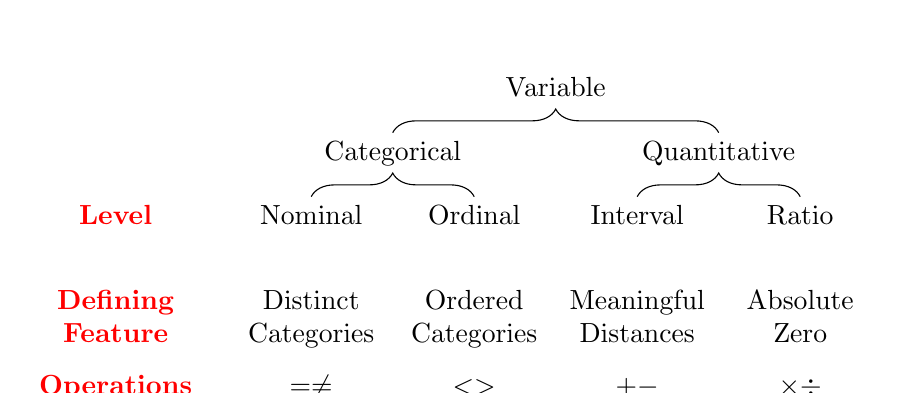
\begin{tikzpicture}[scale=0.9,text height=1.5ex,text depth=.25ex]
  \node (h) at (2.3, 0) {};
  \node (v) at (0,0.8) {};
  \node (Nominal) at (1, 2) {Nominal};
  \node (Ordinal) at ($(Nominal)+(h)$) {Ordinal};
  \node (Interval) at ($(Nominal)+2*(h)$) {Interval};
  \node (Ratio) at ($(Nominal)+3*(h)$) {Ratio};
  \node (Equality) at ($(Nominal)-3*(v)$) {$=\ne$};
  \node (LessMore) at ($(Ordinal)-3*(v)$) {$<>$};
  \node (PlusMinus) at ($(Interval)-3*(v)$) {$+-$};
  \node (MultiplyDivide) at ($(Ratio)-3*(v)$) {$\times\div$};
  \node [text width=2cm,text centered] (Mutual) at ($(Nominal)-1.5*(v)$) {Distinct Categories};
  \node [text width=2cm,text centered] (Order) at ($(Ordinal)-1.5*(v)$) {Ordered Categories};
  \node [text width=2cm,text centered] (Distance) at ($(Interval)-1.5*(v)$) {Meaningful Distances};
  \node [text width=2cm,text centered] (Magnitude) at ($(Ratio)-1.5*(v)$) {Absolute Zero};
  \node [color=red] (Level) at ($(Nominal)-1.2*(h)$) {\textbf{Level}};
  \node [text width=2cm,text centered, color=red] (Feature) at ($(Level)-1.5*(v)$) {\textbf{Defining Feature}}; 
  \node [color=red] (Operation) at ($(Level)-3*(v)$) {\textbf{Operations}}; 
\draw[decoration={brace,amplitude=3mm}, decorate] (Nominal.north) -- (Ordinal.north) node[midway,above=3mm] (Categorical) {Categorical};
  \draw[decoration={brace,amplitude=3mm}, decorate] (Interval.north) -- (Ratio.north) node[midway,above=3mm] (Quantitative) {Quantitative};
    \draw[decoration={brace,amplitude=3mm}, decorate] (Categorical.north) -- (Quantitative.north) node[midway,above=3mm] (Variable) {Variable};
\end{tikzpicture}
\caption{Stevens' levels of measurement}
\label{fig:Stevens}
\end{figure}

\section{Nominal scales}
In a \defword{nominal scale},\marginnote{A \defword{nominal scale} groups observations into unordered categories.} we note only that some things are different from others and that they belong to two or more \defword{mutually exclusive} categories. \marginnote[4mm]{In \defword{mutually exclusive} categories nothing belongs to more than one category (at the same time and in the same sense).}If we say that a person has Down syndrome (trisomy 21), we are implicitly using a nominal scale in which there are people with Down syndrome and people without Down syndrome. In a true nominal scale, there are no cases that fall between categories. To be sure, we might have some difficulty figuring out and reliably agreeing upon the category to which something belongs---but there is no conceptual space between categories.

In the messy world of observable reality, few true nominal variables exist as defined here. Most so-called nominal variables in psychology are merely nominal-\emph{ish}. With respect to Down syndrome, we could say that people either have three copies of the 21\textsuperscript{st} chromosome or they do not. However, if we did say that---and meant it---we'd be wrong. In point of fact, there are many cases of partial trisomy. There are other cases of Down syndrome in which part of chromosome 21 is copied to another chromosome. However, because cases like this are sufficiently rare and because such distinctions are usually not of vital importance, Down Syndrome is treated as if it were a true nominal variable. Even though Down Syndrome might technically come in degrees (both phenotypically and in terms of the underlying chromosomal abnormalities), the distinction between not having the condition and not having it is not \defword{arbitrary}.\marginnote{\defword{Arbitrary} refers to things that are decided not by necessity but by preference, convenience, or whim.} 

\begin{figure}      
  \centering      
      \captionsetup [subfloat]{captionskip=12pt}
    \subfloat [A (nearly) true dichotomy]{
    \centering
    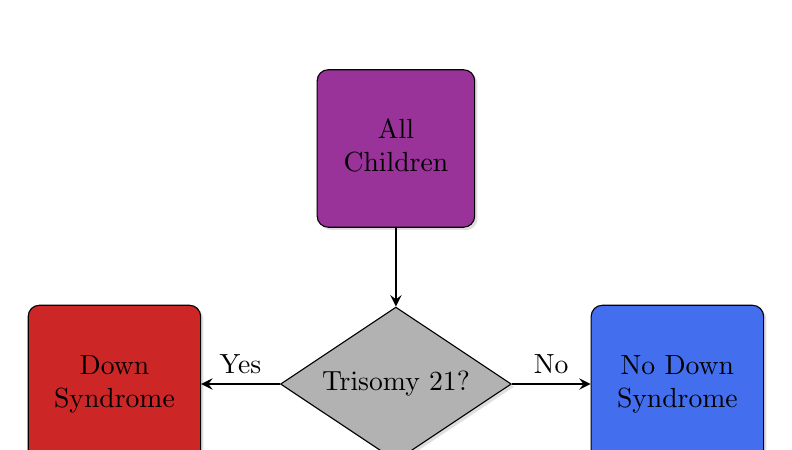
\begin{tikzpicture}
    [node distance=1cm and 1cm]
    \definecolor{firebrick2}{RGB}{205,38,38};
    \definecolor{royalblue2}{RGB}{67,110,238};
    \node [rectangle,rounded corners,minimum size=20mm,fill=violet!80,drop shadow={opacity=0.25,shadow xshift=1pt, shadow yshift=-1pt},draw] (All) at (0,0) {\begin{tabular}{c} All\\Children\end{tabular}};
    \node (Trisomy) [shape=diamond, below= of All,fill=black!30,shape aspect=1.5,drop shadow={opacity=0.25,shadow xshift=1pt, shadow yshift=-1pt},draw] {Trisomy 21?};
    \node [rectangle,rounded corners,minimum size=20mm,fill=firebrick2,drop shadow={opacity=0.25,shadow xshift=1pt, shadow yshift=-1pt},left=of Trisomy,draw] (Down) {\begin{tabular}{c} Down\\Syndrome\end{tabular}};
    \node [rectangle,rounded corners,minimum size=20mm,fill=royalblue2,drop shadow={opacity=0.25,shadow xshift=1pt, shadow yshift=-1pt},right=of Trisomy,draw] (NoDown) {\begin{tabular}{c} No Down\\Syndrome\end{tabular}}; 
    \draw[-stealth,thick] (All) to (Trisomy);
    \draw[-stealth,thick] (Trisomy) -- (Down) node [midway,above] {Yes};
    \draw[-stealth,thick] (Trisomy) -- (NoDown) node [midway,above] {No};
    \end{tikzpicture}
    \label{fig:down}
    }    
  \hspace{.25in}% 
  \captionsetup [subfloat]{captionskip=0pt}
    \subfloat [A dichotomized continuum]{
    \centering
\begin{knitrout}
\definecolor{shadecolor}{rgb}{0.969, 0.969, 0.969}\color{fgcolor}
\includegraphics[width=\maxwidth]{figure/IntellectualDisability} 

\end{knitrout}
    } \\ 
  \caption{Two kinds of dichotomous variables}    
  \label{fig:dichotomous}
\end{figure} 

In contrast, consider the diagnosis of \emph{intellectual disability}, what has historically been called ``mental retardation.'' We might have only two categories in our coding scheme (Intellectual Disability: Yes or No) but it is widely recognized that the condition comes in degrees (e.g., ``none,'' ``borderline,'' ``mild,'' ``moderate,'' ``severe,'' and ``profound''). Thus, intellectual disability is not even conceptually nominal. It is a continuum that has been divided at a convenient but mostly arbitrary point (Figure~\ref{fig:dichotomous}). Distinguishing between a \defword{dichotomous}\marginnote{A \defword{dichotomy} is a division of something into two categories.} variable that is nominal by nature and one that has an underlying continuum matters because there are statistics that apply only to the latter type of variable (e.g., the tetrachoric correlation coefficient). Even so, in many procedures, the two types of dichotomies can be treated identically (e.g., comparing the means of two groups with an independent-samples t-test).


What if the categories in a nominal scale are not mutually exclusive? For example, suppose that we have a variable in which people can be classified as having either Down syndrome or Klinefelter syndrome (XXY). Obviously, this is a \defword{false dichotomy}\marginnote{In a \defword{false dichotomy}, two alternatives are presented as if they are the only alternatives when, in fact, there are others available.}. Most people have neither condition. Well, we can expand the nominal variable to have three categories: Down syndrome, Klinefelter syndrome, and neither. What if a person has both Down syndrome \emph{and} Klinefelter syndrome? Okay, we just add a fourth category: both. This combinatorial approach is not so much a problem for some purposes (e.g., the ABO blood group system), but for many variables, it quickly becomes unwieldy. If we wanted to describe all chromosomal abnormalities with a single nominal variable, the number of combinations increases exponentially with each new category added. This might be okay if having two or more chromosomal abnormalities is very rare. If, however, the categories are not mutually exclusive and combinations are common enough to matter, it is generally easiest to make the variable into two or more nominal variables (Down syndrome: Yes or no; Klinefelter syndrome: Yes or no; Edwards syndrome: Yes or no; and so forth). Some false dichotomies are so commonly used that people know what you mean, even though they are incomplete (e.g., Democrat vs. Republican) or potentially insensitive to people who do not fit neatly into any of the typical categories (e.g., male vs. female).

When we list the categories of a nominal variable, the order in which we do so is mostly arbitrary. In the variable \emph{college major}, no major intrinsically comes before any other. It is convenient to list the categories alphabetically but the order is different in different languages and will change as the names of college majors evolve. However, strict alphabetical order is not always logical or convenient.\sidenote{ For example, in a variable such as \emph{ethnic identity}, the number of possible categories is very large so members of very small groups are given the option of writing in their answer next to the word ``other.'' The ``other'' category is placed at the end of the list to avoid confusion.}

\section{Ordinal scales}
In an \defword{ordinal scale},\marginnote{An \defword{ordinal scale} groups observations into ordered categories.} things are still classified by category but the categories have a particular order. Suppose that we are conducting behavioral observations of a child in school and we record when the behavior occurred. The precise time at which the behavior occurred (e.g., 10:38~AM) may be uninformative. If the class keeps a fairly regular schedule, it might be more helpful to divide the day into categories such as early morning, recess, late morning, lunch, and afternoon. This way it is easy to see if behavior problems are more likely to occur in some settings (or activities) than in others. It does not matter that these divisions are of unequal lengths or that they do not occur at precisely the same time each day. In a true ordinal variable, the distance between categories is either undefined, unspecified, or irrelevant. 

\begin{marginfigure}
\centering
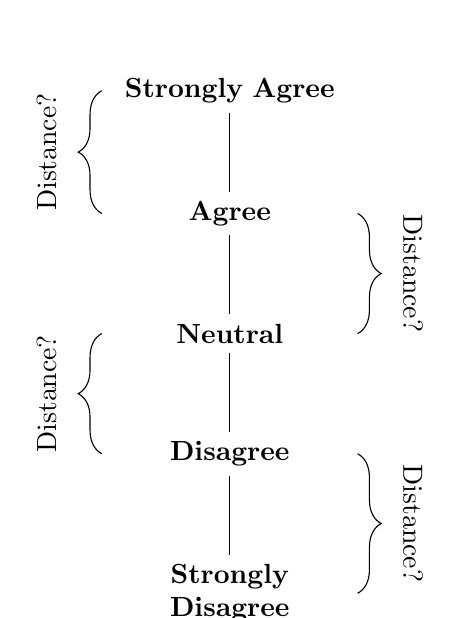
\begin{tikzpicture} [font=\normalsize]
\node [align=center,text width=3cm] (sd)  {\textbf{Strongly Disagree}};
\node [align=center,text width=3cm,above=of sd]  (d) {\textbf{Disagree}};
\node [align=center,text width=3cm,above=of d]  (n) {\textbf{Neutral}}; 
\node [align=center,text width=3cm,above=of n] (a)  {\textbf{Agree}};
\node [align=center,text width=3cm,above=of a] (sa) {\textbf{Strongly Agree}};
\draw [decoration={brace,amplitude=3mm}, decorate] (d.east) -- (sd.east) node[midway, rotate=-90,align=center,yshift=2em]{Distance?};
\draw [decoration={brace,amplitude=3mm}, decorate] (d.west) -- (n.west) node[midway, rotate=90,align=center,yshift=2em]{Distance?};
\draw [decoration={brace,amplitude=3mm}, decorate] (a.east) -- (n.east) node[midway, rotate=-90,align=center,yshift=2em]{Distance?};
\draw [decoration={brace,amplitude=3mm}, decorate] (a.west) -- (sa.west) node[midway, rotate=90,align=center,yshift=2em]{Distance?};
\draw (sd.north) -- (d.south);
\draw (d.north) -- (n.south);
\draw (n.north) -- (a.south);
\draw (a.north) -- (sa.south);
\end{tikzpicture}
\caption{In a Likert-type scale, the distances between categories are undefined.}
\label{fig:Likert}
\end{marginfigure}
Most measurement in psychological assessment involves ordinal scales, though in many cases ordinal scales might appear to be other types of scales. Questionnaires that use Likert-type scales are very clearly ordinal (e.g., Figure~\ref{fig:Likert}). Even though true/false items on questionnaires might seem like nominal scales, they are usually ordinal because the answer indicates whether a person has either more or less of an attribute. That is, \emph{more} and \emph{less} are inherently ordinal concepts. Likewise, ability test items are ordinal, even though \emph{correct} vs. \emph{incorrect} might seem like nominal categories. Ability tests are designed such that a correct response indicates more ability than an incorrect response. The ordinal nature of ability test items is especially clear in cases that allow for partial credit. 

Some scales are only partially ordinal. For example, \emph{educational attainment} is ordinal up to a certain point in most societies, but branches out as people acquire specialized training. For a career in psychology, the educational sequence is high school diploma, associate's degree, bachelor's degree, master's degree, and doctoral degree.\sidenote{Obviously, some of these degrees can be skipped and the endpoint is different for different careers in psychology. Furthermore, not all degrees fit neatly in this sequence (e.g., the school psychology specialist degree).} However, this is not the sequence for real estate agents, hair stylists, and pilots. If we wanted to compare educational degrees across professions, how would we rank them? For example, how would we compare a law degree with a doctorate in geology? Are they the same? Does one degree indicate higher educational attainment than the other? The answers depend on the criteria that we care about---and different people care about different things. Thus, it is difficult to say that we have an ordinal scale when we compare educational attainment across professions. 

\begin{figure} 
% \centering
\begin{knitrout}
\definecolor{shadecolor}{rgb}{0.969, 0.969, 0.969}\color{fgcolor}
\includegraphics[width=\maxwidth]{figure/differentiation} 

\end{knitrout}
\caption{Anxiety is more differentiated at higher levels of distress}
\label{fig:differentiation}
\end{figure}

Like educational attainment, many psychological traits are more differentiated at some points in the continuum than at others. For example, as seen in Figure~\ref{fig:differentiation}, it sometimes convenient to lump the various flavors of trait anxiety together at the low and middle range of distress and then to distinguish among them at the high end. It is difficult to say who is more anxious, a person who is extremely paranoid\sidenote{Although \emph{paranoia} is not traditionally considered a type of anxiety, it is clear that anxiety (about the possibly malevolent intentions of others) is a core feature of the trait.} or a person with a severe case of panic disorder. We can say that each is more anxious than the average person (an ordinal comparison) but each has a qualitatively different kind of anxiety. This problem is easily solved by simply talking about two different scales (paranoia and panic). However, there are different kinds of paranoia (e.g., different mixtures of hostility, fear, and psychosis) and different kinds of panic (e.g., panic vs. fear of panic). One can always divide psychological variables into ever narrower categories, making comparisons among and across related constructs problematic. At some point, we gloss over certain qualitative differences and treat them as if they were comparable, even though, strictly speaking, they are not.

\section{Interval scales}
With \defword{interval scales},\marginnote{In an \defword{interval scale} the distance between numbers has a consistent meaning at every point on the scale.} not only are the numbers on the scale ordered, the distance between the numbers (i.e., intervals) is meaningful. A good example of an interval scale is the calendar year. The time elapsed from 1960 to 1970 is the same as the time elapsed from 1970 to 1980. In contrast, consider a standard Likert scale from a questionnaire. What is the distance between \emph{disagree} and \emph{agree}? Is it the same as the distance between \emph{agree} and \emph{strongly agree}? If it were, how would we know? In interval scales, all such mysteries disappear. 

It is not always easy to distinguish between an interval scale and an ordinal scale. Therapists sometimes ask clients to rate their distress "on a scale from 0 to 10." Probably, in the mind of the therapist, the distance between each point of the scale is equal. In the mind of the client, however, it may not work that way. In Figure~\ref{fig:suds}, a hypothetical client thinks of the distance between 9 and 10 as much greater than the distance between 0 and 1. \begin{marginfigure} 
\centering
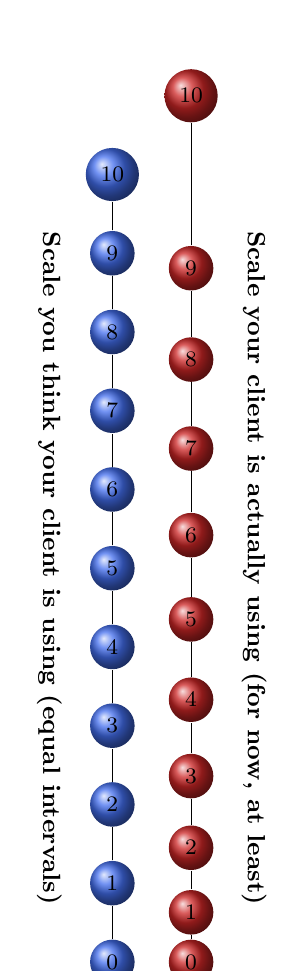
\begin{tikzpicture}[scale=1]
    \definecolor{firebrick2}{RGB}{205,38,38};
    \definecolor{royalblue2}{RGB}{67,110,238};
   \pgfmathtruncatemacro{\T}{10}
   \tikzstyle{every node}=[draw=none,shape=circle,ball color=royalblue2,minimum size=5.5mm];
   \foreach \n in {0,...,\T} 
      \node (\n) at (0,\n) {\footnotesize{\n}};
   \foreach \n [remember=\n as \lastn (initially 0)] in {0,...,\T} 
      \draw (\lastn) -- (\n);
   \tikzstyle{every node}=[draw=none,shape=circle,ball color=firebrick2,minimum size=5.5mm];
\def\myarray{{0,0.63,1.45,2.36,3.33,4.35,5.42,6.52,7.65,8.81,11}};
   \foreach \x [count=\xi] in {0,...,10} 
      \node (\x) at (1,\myarray[\x]) {\footnotesize{\x}};
   \foreach \x [remember=\x as \lastx (initially 0)] in {0,...,\T} 
      \draw (\lastx) -- (\x);
   \tikzstyle{every node}=[rotate=-90];
\node at (-0.8,5) {\textbf{\small{Scale you think your client is using (equal intervals)}}};
\node at (1.8,5) {\textbf{\small{Scale your client is actually using (for now, at least)}}};
 \end{tikzpicture} 
\caption{Subjective units of distress may not be of equal length}
\label{fig:suds}
% %<<SUDS,fig.width=5, fig.height=5, echo = FALSE,crop=TRUE,cache=TRUE,fig.keep='high'>>=
% # p<-seq(0.2,.99,.79/10)
% # plot(qnorm(seq(0.2,0.99,0.005))~seq(0.2,0.99,0.005),type='l',xlab="Scale Intended by the Clinician",ylab="How a Client Might Use the Scale",axes=FALSE,lwd=1,col="gray")
% # axis(1, at = p,label=0:10)
% # axis(2, at = z,label=0:10,las=2)
% # points(p,sz,type="p",lwd=1,col="black",pch = 19)
% %@
\end{marginfigure} 

It is doubtful that any subjectively scaled measurement is a true interval scale. Even so, it is clear that some ordinal scales are more interval-like than others. Using item response theory \citep{embretson2000item}, it is possible to sum many ordinal-level items and scale the total score such that it approximates an interval scale. It is important to note, however, that item response theory does not accomplish magic. The application of item response theory in this way is justified only if the ordinal items are measuring an underlying construct that is by nature at the interval (or ratio) level. No amount of statistical wizardry can alter the nature of the underlying construct. Sure, you can apply fancy math to the numbers, but a construct that is ordinal by nature will remain ordinal no matter what you do or convince yourself that you have done.

Most of the tools used in psychological assessment make use of ordinal scales and transform them such that they are treated as if they were interval scales. Is this defensible? Yes, a defense is possible \citep[e.g.,][]{borsboom2004psychometrics} but not all scholars will be convinced by it \citep{michell1997quantitative,michell2008psychometrics}. As an act of faith, I will assume that most of the scales used in psychological assessment (measures of abilities, personality traits, attitudes, interests, motivation, and so forth) are close enough to interval scales that they can be treated as such. In many instances, my faith may be misplaced, but where exactly can only be determined by high quality evidence. While I await such evidence, I try to balance my faith with moderate caution.

\section{Ratio scales}
In a \defword{ratio scale},\marginnote{A \defword{ratio scale} has a true zero, in addition to all the properties of an interval scale.} zero represents something special: the absence of the quantity being measured. In an interval scale, there may be a zero, but the zero is just another number in the scale. For example, $0\,^{\circ}\mathrm{C}$ happens to be the freezing point of water at sea level but it does not represent the absence of heat.\sidenote{The absence of heat occurs at $-273.15\,^{\circ}\mathrm{C}$ or $0\,^{\circ}\mathrm{K}$.} Ratio scales do not usually have negative numbers but there are exceptions.\sidenote[][4mm]{For example, in a checking account balance, negative numbers indicate that the account is overdrawn. Still, a checking account balance is a true ratio scale because a zero indicates that there is no money in the account.}

What does a true zero have to do with ratios? In interval scales, numbers can be added and subtracted but they cannot be sensibly divided. Why not? Because when you divide one number by another, you are creating a ratio. A ratio tells you how big one number is compared to another number. Well, how big is any number? The magnitude of a real number is its distance from zero (i.e., its absolute value). If zero is not a meaningful number on a particular scale, then ratios computed from numbers on that scale will not be meaningful. Therefore, because interval scales do not have a true zero, meaningful ratios are not possible. For example, although $20\,^{\circ}\mathrm{C}$ is twice as far from $0\,^{\circ}\mathrm{C}$ as $10\,^{\circ}\mathrm{C}$, it does not mean that $20\,^{\circ}\mathrm{C}$ is twice as hot as $10\,^{\circ}\mathrm{C}$. In contrast, these types of comparisons are possible on the Kelvin scale because $0\,^{\circ}\mathrm{K}$ is a true zero. That is, $20\,^{\circ}\mathrm{K}$ really is twice as hot as $10\,^{\circ}\mathrm{C}$.

In psychological assessment, there are a few true ratio scales that are commonly used. Whenever anything is counted (e.g., counting how often a behavior occurs in a direct observation), it is a ratio scale. However, this is a bit tricky. If I observe how many times a child speaks out of turn in class and I use this as an index of impulsivity, it is no longer a ratio scale. Why? Well, the actual variable, \emph{number of outbursts} is a true ratio variable because 0 outbursts means the absence of outbursts. However, if I use the number of outbursts as a proxy variable for \emph{impulsivity}, then 0 outbursts probably does not indicate the absence of impulsivity. At best it indicates lower levels of impulsivity. This same problem exists for the measurement of reaction times. Reaction time is a true ratio because a reaction time of 0 means that no time has elapsed between the onset of the stimulus and the response. However, reaction time data used in clinical applications are often proxies for traits that are interval-level concepts, such as \emph{inattention} on a continuous performance test. Why are psychological traits such as cognitive abilities, personality traits, and so forth interval-level concepts? Because we do not yet have any means of defining what, for example, zero intelligence or zero extraversion would look like. Attempts have been made \citep{jensen2006clocking}, but they have not yet proved persuasive.

\section{Discrete vs. Continuous Variables}\label{sec:DiscreteVsContinuous}
Interval and ratio variables can be either discrete or continuous. \defword{Discrete variables}\marginnote{A \defword{discrete variable} can only take on exact values from a specified list.} can assume some values but not others. Once the list of acceptable values has been specified, there are no cases that fall between those values. For example, the number of bicycles a person owns is a discrete variable because the variable can assume only the non-negative integers. Fractions of bicycles are not considered. Discrete variables usually take on integer values but this is not necessarily the case. 

\begin{figure}
\centering
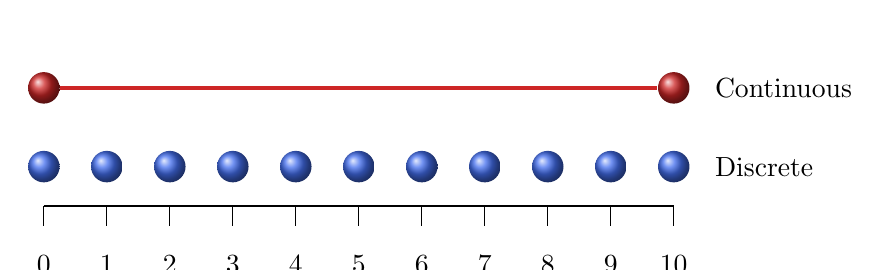
\begin{tikzpicture}[xscale=0.8]
    \definecolor{firebrick2}{RGB}{205,38,38};
    \definecolor{royalblue2}{RGB}{67,110,238};
\node [anchor=west] at (10.5,1.25) {Discrete};
\node [anchor=west] at (10.5,2.25) {Continuous};
\foreach \n in {0,...,10} {
    \node at (\n,0) {\n};
    \draw (\n,0.5)--(\n,0.75);
  }
 \tikzstyle{every node}=[draw=none,shape=circle,ball color=royalblue2,minimum size=4mm];
\foreach \n in {0,...,10} {
    \node at (\n,1.25) {};
}
\draw (0,0.75) --(10,0.75);
 \tikzstyle{every node}=[draw=none,shape=circle,ball color=firebrick2,minimum size=4mm];
\node (r1) at (0,2.25) {};
\node  (r10)  at (10,2.25) {};
\draw [color=firebrick2,ultra thick] (r1.east)--(r10.west);
\end{tikzpicture}
\caption{Discrete variables have gaps whereas continuous variables have none.}
\label{fig:DiscreteContinuous}
\end{figure}

When a variable can assume any value within a specified interval, the variable is said to be \defword{continuous}.\marginnote{A \defword{continuous variable} can take on any value within a specified range.} In theory, this means that fractions and decimals can be used to achieve any level of precision that we desire. In practice, we must round the numbers at some point, technically making the variable discrete. In truly discrete variables, however, we could not change our minds and decide to round the numbers such that they are more precise.


% !Rnw root = Test.Rnw
\chapter{Probability Distributions}
\section{Random Variables}
Because we first learn about variables in an algebra class, we tend to think of variables as having values that can be solved for---if we have enough information about them. Algebraic variables are ``determined'' by constraints---in the form of equations.\sidenote{If I say that $x$ is a variable and that $x+6=8$, that equation constrains $x$ so that it must be exactly $2$, no more and no less. What about when there are two variables and one equation, such as $x+y=10$? Isn't $x$ free to be any value? Yes, but even here, $x$ is still constrained by $y$. Once one variable is determined, the other is also determined. If $y$ is $3$, then $x$ must be $7$. In other words, because of the constraint of the equation, there is only one degree of freedom, meaning that only one of the two variables is free to vary at a time.}

\defword{Random variables}\marginnote{\defword{Random variables} have values that are determined by a random process.} are not like algebraic variables. Random variables simply take on values because of some random process. If we say that the outcome of a throw of a six-sided die is a random variable, there is nothing to ``solve for.'' There is no equation that determines the value of the die. Instead, it is determined by chance and the physical constraints of the die. That is, the outcome must be one of the numbers printed on the die and the six numbers are equally likely to occur (if the die is ``fair''). This illustrates an important point. The word \emph{random} here does not mean ``anything can happen.'' Random variables have outcomes that are subject to random processes, but those random processes \emph{do}  have constraints on them such that some outcomes are more likely than others---and some outcomes never occur at all.

When we say that the throw of a six-sided die is a random variable, we are not talking about any particular throw of a particular die but, in a sense, \emph{every} throw (that has ever happened or ever could happen) of \emph{every} die (that has ever existed or could exist). Imagine an immense, roaring, never-ending, cascading flow of dice falling from the sky and a giant scoreboard nearby recording the relative frequencies of ones, twos, threes, fours, fives, and sixes as each die lands and then disappears. That's a random variable.

\section{Sample Spaces}\label{sec:SampleSpace}

The set of all possible outcomes of a random variable is the \defword{sample space}.\marginnote{A \defword{sample space} is the set of all possible values that a random variable can assume.} Continuing with our example, the sample space of a single throw of a six-sided die is the set $\big\{$\tikz [baseline=.125ex]{\drawdie [scale=0.8]{1}},\tikz [baseline=.125ex]{\drawdie [scale=0.8]{2}},\tikz [baseline=.125ex]{\drawdie [scale=0.8]{3}},\tikz [baseline=.125ex]{\drawdie [scale=0.8]{4}},\tikz [baseline=.125ex]{\drawdie [scale=0.8]{5}},\tikz [baseline=.125ex]{\drawdie [scale=0.8]{6}}$\big\}$. \emph{Sample space} is a curious term. Why \emph{sample} and why \emph{space}? With random variables, \defword{populations}\marginnote{A \defword{population} consists of all entities under consideration.} are infinitely large, at least theoretically. Random variables just keep spitting out numbers forever! So any time we actually observe numbers generated by a random variable, we are always observing a \defword{sample};\marginnote{A \defword{sample} is a subset of a population.} actual infinites cannot be observed in their entirety. A \defword{space} is a set that has mathematical structure. Most random variables generate either integers or real numbers, both of which are structured in many ways (e.g., order).

Unlike distributions having to do with dice, many distributions have a sample space with an infinite number of elements. Actually there are two kinds of infinity we can consider. One distribution we will discuss later is the Poisson distribution. Its sample space is the set of whole numbers: \{0,1,2,...\}, which extends to positive infinity. The sample space of continuous variables is infinitely large for another reason. Between any two points in a continuous distribution, there is an infinite number of other points. For example, in the continuous uniform distribution, the sample space consists of all real numbers between two points. Many continuous distributions have sample spaces that involve both kinds of infinity. For example, the sample space of the normal distribution consists of all real numbers from negative infinity to positive infinity.

\section{Probability Distributions}\label{sec:ProbabilityDistribution}

\begin{marginfigure}
\begin{center}
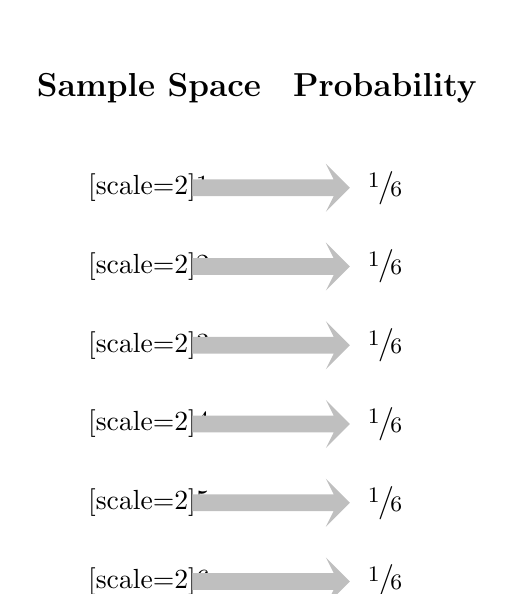
\begin{tikzpicture}
\foreach \n in {1,...,6} {
\node at ($(0,7)-(0,\n)$) {\drawdie [scale=2]{\n}};
\node [fill=gray!50, minimum height=2cm, minimum width=0.1cm, single arrow, single arrow head extend=.2cm, single arrow head indent=.1cm, inner sep=1mm] at ($(1.5,7)-(0,\n)$) {};
\node  (p1) at (3,\n) {\large{$\sfrac{1}{6}$}};
}
  \node [text centered,anchor=south,text height=1.5ex,text depth=.25ex] (p3) at (0,7) {\large{\textbf{Sample Space}}};
  \node [text centered,anchor=south,text height=1.5ex,text depth=.25ex] (p4) at (3,7) {\large{\textbf{Probability}}};
 \end{tikzpicture}
\caption{The probability distribution of a throw of a single die}
\label{fig:dice}
\end{center}
\end{marginfigure}

Each element of a random variable's sample space has some probability associated with it. When we list the probabilities of each possible outcome, we have specified the variable's \defword{probability distribution}\marginnote[4mm]{In a \defword{probability distribution}, there is an assignment of a probability to each possible element in a variable's sample space.}. In other words, if we know the probability distribution of a variable, we know how probable each outcome is. In the case of a throw of a single die, each outcome is equally likely (Figure~\ref{fig:dice}). 

There is an infinite variety of probability distributions, but a small subset of them have been given names. Now, one can manage one's affairs quite well without ever knowing what a Bernoulli distribution is, or what a $\chi{^2}$ distribution is, or even what a normal distribution is. However, sometimes life is a little easier if we have names for useful things that occur often. Most of the distributions with names are not really single distributions, but families of distributions. The various members of a family are unique but they are united by the fact that their probability distributions are generated by a particular mathematical function (more on that later). In such cases, the probability distribution is often represented by a graph in which the sample space is on the $X$-axis and the associated probabilities are on the $Y$-axis. In Figure~\ref{fig:pdfIllustration}, 16 probability distributions that might be interesting and useful to clinicians are illustrated. Keep in mind that what are pictured are only particular members of the families listed; some family members look quite different from what is shown in Figure~\ref{fig:pdfIllustration}.

\begin{figure*}
\centering
\begin{knitrout}
\definecolor{shadecolor}{rgb}{0.969, 0.969, 0.969}\color{fgcolor}
\includegraphics[width=\maxwidth]{figure/pdfIllustration} 

\end{knitrout}
\caption{A gallery of useful distributions}
\label{fig:pdfIllustration}
\end{figure*}

\section{Discrete Uniform Distributions}\label{sec:DiscreteUniform}

The throw of a single die is a member of a family of distributions called the \defword{discrete uniform distribution}.\marginnote{A \defword{discrete uniform distribution} is a family of random variable distributions in which the sample space is an evenly spaced sequence of numbers, each of which is equally likely to occur.} It is ``discrete'' because the elements in the sample space are countable, with evenly spaced gaps between them. For example, there might be a sequence of 8, 9, 10,and 11 in the sample space but there are no numbers in between. It is ``uniform'' because all outcomes are equally likely. With dice, the numbers range from a lower bound of 1 to an upper bound of 6. In the family of discrete uniform distributions, the lower and upper bounds are typically integers, mostly likely starting with 1. However, any real number $a$ can be the lower bound and the spacing $k$ between numbers can be any positive real number. For the sake of simplicity and convenience, I will assume that the discrete uniform distribution refers to consecutive integers ranging from a lower bound of $a$ and an upper bound of $b$. 

This kind of discrete uniform distribution has a number of characteristics listed below. I will explain each of them in the sections that follow.\marginpar{As we go, I will also explain the mathematical notation. For example, $a \in \mathbb{Z}$ means that $a$ is an integer because $\in$ means \emph{is a member of} and $\mathbb{Z}$ is the set of all integers.}

\begin{equation*}
\boxed{
\setlength{\extrarowheight}{3pt}
\begin{array}{rccc}
%\text{\textbf{Discrete Uniform Distribution}}&&\\
\text{Lower Bound:} & a  & \hyperref [note:In]{\in} &\hyperref [note:Z]{\mathbb{Z}}\\
\text{Upper Bound:} & b & \in & \mathbb{Z}\\
&&&b>a\\
\text{Sample Space:} & x &\in&\{a,a+1,\hdots,b\}\\
\text{Number of points:} & n&=&b-a+1 \\
\text{Mean:} & \mu&=&\frac{a+b}{2} \\
\text{Variance:} & \sigma^2&=&\frac{n^2-1}{12} \\
\text{Skewness:} & \gamma_1&=&0 \\
\text{Kurtosis:} & \gamma_2&=&-\frac{6(n^2+1)}{5(n^2-1)} \\
\text{Probability Mass Function:} & f_X(x;a,b)&=&\frac{1}{n} \\
\text{Cumulative Distribution Function:} & F_X(x;a,b)&=&\frac{x-a+1}{n} \\
\end{array}
}
\end{equation*}

\section{Parameters of Random Variables}
The lower bound $a$, the spacing between numbers $k$, and the number of points $n$ are the discrete uniform distribution's \defword{parameters}.\marginnote{A \defword{parameter} is a defining feature of a random variable's probability distribution.} If we restrict ourselves to the more common case in which the sample space consists of consecutive integers, we can say that the parameters are simply the lower bound $a$ and the upper bound $b$. The word \emph{parameter} has many meanings but here it refers to a characteristic of a distribution family that helps us identify precisely which member of the family we are talking about. Most distribution families have one, two, or three parameters. 

If you have taken an algebra class, you have seen parameters before, though the word \emph{parameter} many not have been used. Think about the formula of a line:
\begin{equation*}\label{eq:linear}
y=mx+b
\end{equation*}
Both $x$ and $y$ are variables, but what are $m$ and $b$? Well, you probably remember that $m$ is the slope of the line and that $b$ is the $y$-intercept. If we know the slope and the intercept of a line, we know exactly which line we are talking about. No additional information is needed to graph the line. Therefore, $m$ and $b$ are the line's \emph{parameters}, because they uniquely identify the line.\sidenote{What about other mathematical functions? Do they have parameters? Yes! All of them do! For example, in the equation for a parabola ($y=ax^2+bx+c$), $a$, $b$, and $c$ determine its precise shape.} All lines have a lot in common but there is an infinite variety of lines because the parameters, the slope and the intercept, can take on the value of any real number. Each unique combination of parameter values (slope and intercept) will produce a unique line. So it is with probability distribution families. All family members are alike in many ways but they also differ because of different parameter values.

The discrete uniform distribution (i.e., the typical variety consisting of consecutive integers) is defined by the lower and upper bound. Once we know the lower bound and the upper bound, we know exactly which distribution we are talking about.\sidenote{If we allow the lower bound to be any real number and the spacing to be any positive real number, the discrete uniform distribution can be specifed by three parameters: the lower bound $a$, the spacing between numbers $k$ ($k>0$), and the number of points $n$ ($n$>1). The upper bound $b$ of such a distribution would be $b=a+k(n-1)$} Not all distributions are defined by their lower and upper bounds. Indeed, many distribution families are unbounded on one or both sides. Therefore, other features are used to characterize the distributions, such as the population mean.

\section{Probability Mass Functions}\label{sec:pmf}
Many distribution families are united by the fact that their probability distributions are generated by a particular mathematical function. For discrete distributions, those functions are called \defword{probability mass functions}.\marginnote{A \defword{probability mass function (pmf)} is a mathematical expression that gives the probability that a discrete random variable will equal a particular element of the variable's sample space.} In general, a mathematical function is an expression that takes one or more constants (i.e., parameters) and one or more input variables, which are then transformed according to some sort of rule to yield a single number.

A probability mass function transforms a random variable's sample space elements into probabilities. In Figure~\ref{fig:dice}, the probability mass function can be thought of as the arrows between the sample space and the probabilities. That is, the probability mass function is the thing that was done to the sample space elements to calculate the probabilities. In Figure~\ref{fig:dice}, each outcome of a throw of the the die was mapped onto a probability of  $\sfrac{1}{6}$. Why $\sfrac{1}{6}$, and not some other number? The probability mass function of the discrete uniform distribution tells us the answer. 

\begin{figure}
\centering
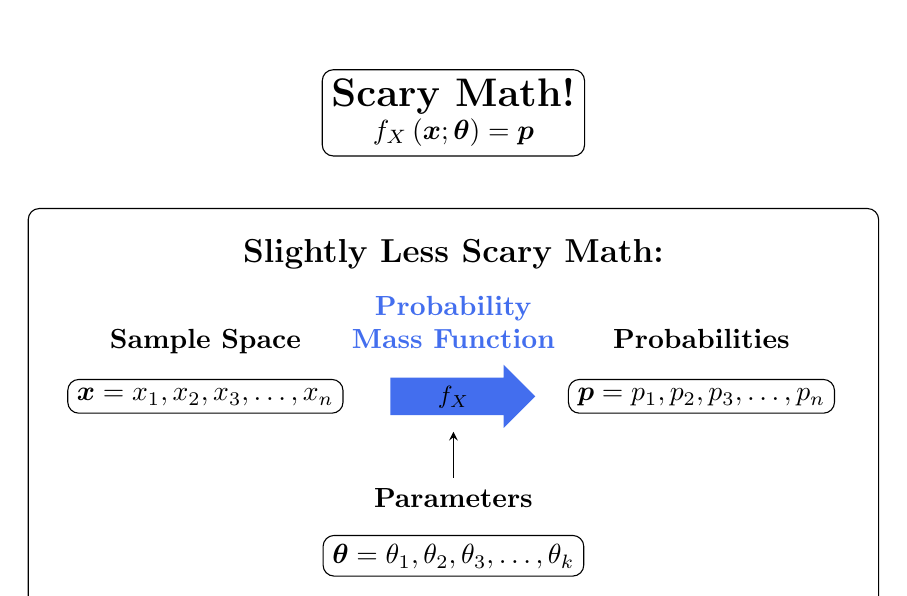
\begin{tikzpicture}[>=stealth,scale=0.9]
\definecolor{firebrick2}{RGB}{205,38,38};
\definecolor{royalblue2}{RGB}{67,110,238};
\node [rectangle,draw, rounded corners,text depth=0.25ex](ss) at (0,0) {$\boldsymbol{x}=x_1,x_2,x_3,\ldots,x_n$};
\node [rectangle,draw, rounded corners,text depth=0.25ex](ps) at (7,0) {$\boldsymbol{p}=p_1,p_2,p_3,\ldots,p_n$};
\node [single arrow,fill=royalblue2,single arrow head extend=1.2ex,transform shape,minimum height=0.9cm,text depth=0.25ex] (fx) at (3.5,0) {$\quad\;\; f_X\quad\;\;$};
\node [text depth=2.25ex,text height= 5ex,anchor=south,yshift=-3.5ex](sst) at (0,0.75) {\textbf{Sample Space}};
\node [text depth=2.25ex,text height= 5ex,anchor=south,yshift=-3.5ex](pst) at (7,0.75) {\textbf{Probabilities}};
\node [shape=rectangle,text depth=2.25ex,color=royalblue2,align=center,text height= 5ex,anchor=south,yshift=-3.5ex](pmf) at (3.5,0.75) {\textbf{Probability}\\
\textbf{Mass Function}};
\node [text depth=2.25ex,text height= 5ex,anchor=south,yshift=-3.5ex] (pt) at (3.5,-1.5) {\textbf{Parameters}};
\draw[->] (3.5,-1.15) to (3.5,-0.5);
\node [rectangle,draw, rounded corners,text depth=0.25ex] (pts) at (3.5,-2.25) {$\boldsymbol{\theta}=\theta_1,\theta_2,\theta_3,\ldots,\theta_k$};
\node [align=center,shape=rectangle,rounded corners,draw](formula) at (3.5,4) {\textbf{\Large{Scary~Math!}}\\
$f_X\left(\boldsymbol{x};\boldsymbol{\theta}\right)=\boldsymbol{p}$};
\draw [rounded corners] (-2.5,-3) rectangle (9.5,2.65);
\node at (3.5,2) {\textbf{\large{Slightly Less Scary Math:}}};
\end{tikzpicture}
\caption{Though one may be scarier than the other, both boxes mean the same thing: Probability mass functions tell us how probable each sample space element is.}
\label{fig:pmf}
\end{figure}

The probability mass function of the discrete uniform distribution is fairly simple but the notation can be intimidating at first (Figure~\ref{fig:pmf}). By convention, a single random variable is denoted by a capital letter $X$. Any particular value of $X$ in its sample space is represented by a lowercase $x$. In other words, $X$ represents the variable in its totality whereas $x$ is merely one value that $X$ can take on. Confusing? Yes, statisticians very work hard to confuse us---and most of the time they succeed! 

The probability mass function of random variable $X$ is denoted by $f_X(x)$. This looks strange at first. It means, "When random variable $X$ generates a number, what is the probability that the outcome will be a particular value $x$?" That is, $f_X(x)=P(X=x)$, where $P$ means "What is the probability that...?" Thus, $P(X=x)$ reads, "What is the probability that random variable $X$ will generate a number equal to a particular value $x$?" So, $f_X(7)$ reads, "When random variable $X$ generates a number, what is the probability that the number will equal 7?"

Most probability mass functions also have parameters, which are listed after a semi-colon. In the case of the discrete uniform distribution consisting of consecutive integers, the lower and upper bounds $a$ and $b$ are included in the function's notation like so: $f_X(x;a,b)$. This reads, "For random variable $X$ with parameters $a$ and $b$, what is the probability that the outcome will be $x$?" Some parameters can be derived from other parameters, as was the case with the number of points $n$ in the sample space of a discrete uniform distribution: $n=b-a+1$. The probability for each outcome in the sample space is the same and there are $n$ possible outcomes. Therefore, the probability associated with each outcome is $\sfrac{1}{n}$.

Putting all of this together, if $a$ and $b$ are integers and $a<b$, for all $n$ integers $x$ between $a$ and $b$,inclusive:
\begin{equation}
f_X(x;a,b)=\frac{1}{b-a+1}=\frac{1}{n}
\end{equation}
Where
\begin{conditions*}
X & A random variable with a discrete uniform distribution\\
f_X & The probability mass function of $X$\\
x & Any particular member of the sample space of $X$\\
a & The lower bound of the sample space\\
b & The upper bound of the sample space\\
n & The number of points in the sample space
\end{conditions*}
You might notice that $x$ is not needed to calculate the probability. Why? Because this is a \emph{uniform} distribution. No matter which sample space element $x$ we are talking about, the probability associated with it is always the same. In all distributions that are not uniform, the position of $x$ matters and thus influences the probability of its occurrence.

\section{Cumulative Distribution Functions}\label{sec:CumDist}
The \defword{cumulative distribution function}\marginnote{A \defword{cumulative distribution function (cdf)} is a mathematical expression that gives the probability that a random variable will equal a particular element of the variable's sample space or less.} tells us where a sample space element ranks in a distribution. Whereas the probability mass function tells us the probability that a random variable will generate a particular number, the cumulative distribution function tells us the probability that a random variable will generate a particular number or less. The cumulative distribution function of the roll of a die (Figure~\ref{fig:cdfDie}) tells us that the probability of rolling at least a \drawdie [scale=0.8]{4} is $\sfrac{4}{6}$ (i.e., $\sfrac{2}{3}$).
\begin{figure}
\centering
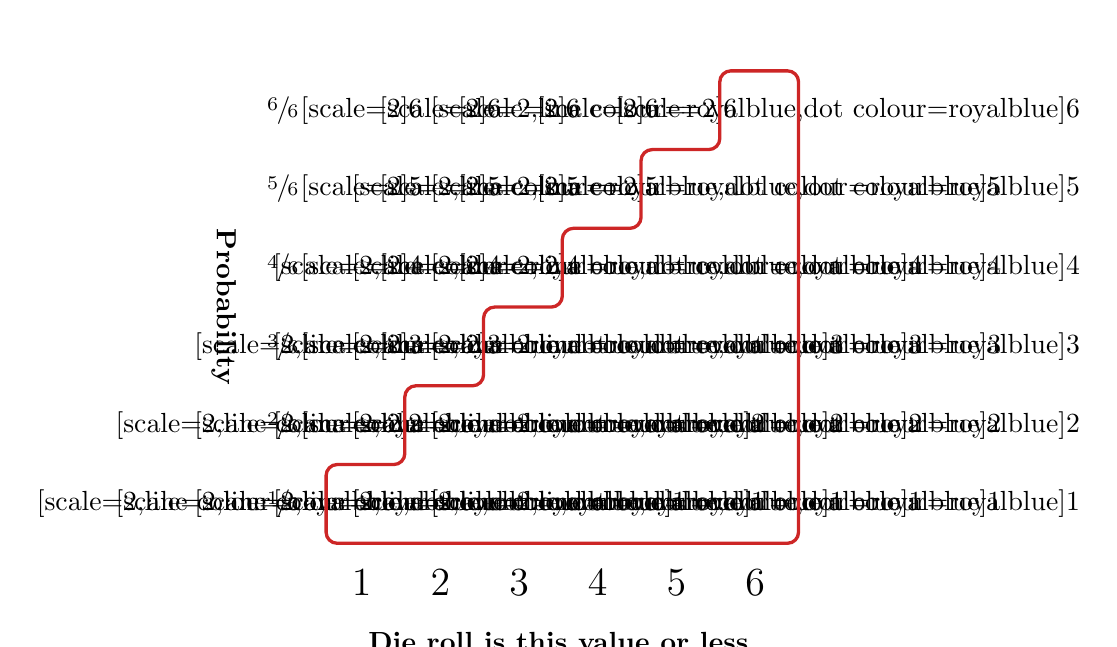
\begin{tikzpicture}
\foreach \i in {1,...,6} {
  \node at (0,\i){$\sfrac{\i}{6}$};
  \node at (\i,0){\Large{\i}};
  \foreach \j in {1,...,6} {
  \ifnum \j>\i
    \node at (\i,\j) {\drawdie [scale=2]{\j}};
  \else
    \node at (\i,\j) {\drawdie [scale=2,line colour=royalblue,dot colour=royalblue]{\j}};
  \fi
  }
}

\draw [firebrick,very thick,rounded corners] (0.55,0.5)-- ++(0,1)-- ++(1,0)-- ++(0,1)-- ++(1,0)-- ++(0,1)-- ++(1,0)-- ++(0,1)-- ++(1,0)-- ++(0,1)-- ++(1,0)-- ++(0,1)-- ++(1,0)-- ++(0,-6)--cycle;
\node[rotate=-90] at (-0.75,3.5) {\textbf{Probability}};
\node at (3.5,-0.75) {\textbf{Die roll is this value or less}};
\end{tikzpicture}
\caption{The cumulative distribution function of the roll of a die is $F_X(x)=\frac{x}{6}$}.
\label{fig:cdfDie}
\end{figure}

The cumulative distribution function is often distinguished from the probability mass function with a capital $F$ instead of a lowercase $f$. In the case of a discrete uniform distribution consisting of $n$ consecutive integers from $a$ to $b$, the cumulative distribution function is:
\begin{equation}
F_X(x;a,b)=\frac{x-a+1}{b-a+1}=\frac{x-a+1}{n}
\end{equation}
Where
\begin{conditions*}
X & A random variable with a discrete uniform distribution\\
F_X & The cumulative distribution function of $X$\\
x & Any particular member of the sample space of $X$\\
a & The lower bound of the sample space\\
b & The upper bound of the sample space\\
n & The number of points in the sample space
\end{conditions*}

\section{Quantile functions}\label{sec:Quantile}

The inverse of the cumultive distribution function is the \defword{quantile function}.\marginnote{A \defword{quantile function} tells us which value in the sample space of a random variable is greater than a particular proportion of the values the random variable generates.} The cumulative distribution starts with a value $X$ in the sample space and tells us $p$, the proportion of values in that distribution that are less than or equal to $X$. A quantile function starts with a proportion $p$ and tells us the value $X$ that splits the distribution such that the proportion $p$ of the distribution is less than or equal to $X$. As seen in Figure~\ref{fig:quantile}, if you see a graph of a continuous distribution function, just flip the X and Y axes and you have a graph of a quantile function!

\begin{figure*}
\centering
\begin{knitrout}
\definecolor{shadecolor}{rgb}{0.969, 0.969, 0.969}\color{fgcolor}
\includegraphics[width=\maxwidth]{figure/QuantileFunction} 

\end{knitrout}
\caption{The quantile function is the inverse of the cumulative distribution function: Just flip the X and Y axes!}
\label{fig:quantile}
\end{figure*}

\section{Generating a Random Sample in Excel and R}

To generate a number from the discrete uniform distribution in Excel, use the \textsf{RANDBETWEEN} function. For example, to generate a random number between 1 and 100, in any cell type:\\
\textsf{=RANDBETWEEN(1,100)}\\
This cell can be copied as many times as is needed to generate a random sample.

In R, the \texttt{runif} function generates numbers from the \hyperref [sec:Uniform] {continuous uniform distribution}. To make the distribution discrete, the \texttt{ceiling} function rounds the numbers up to the nearest integer.\sidenote{A common mistake is to use traditional rounding (up \textsc{or} down to the nearest integer), which makes the lower and upper bounds only half as likely to occur as all the numbers in between.}

\begin{knitrout}
\definecolor{shadecolor}{rgb}{0.969, 0.969, 0.969}\color{fgcolor}\begin{kframe}
\begin{alltt}
\hlcom{# n = the sample size}
\hlstd{n} \hlkwb{<-} \hlnum{1000}
\hlcom{# a = the lower bound}
\hlstd{a} \hlkwb{<-} \hlnum{1}
\hlcom{# b = the upper bound}
\hlstd{b} \hlkwb{<-} \hlnum{100}
\hlcom{# s = the sample with a discrete uniform}
\hlcom{# distribution The runif function generates a}
\hlcom{# number from the continuous uniform distribution.}
\hlcom{# The ceiling function rounds up to the nearest}
\hlcom{# integer.}
\hlstd{s} \hlkwb{<-} \hlkwd{ceiling}\hlstd{(}\hlkwd{runif}\hlstd{(n, a} \hlopt{-} \hlnum{1}\hlstd{, b))}
\hlcom{# Generate a bare-bones plot of the frequency}
\hlcom{# distribution of the sample}
\hlkwd{hist}\hlstd{(s)}
\end{alltt}
\end{kframe}
\end{knitrout}

\section{Bernoulli Distributions}\label{sec:BernoulliDist}
\marginpar{\textbf{Notation notes:}\\
$\lbrack a,b\rbrack $ is the set of all real numbers in the interval between $a$ and $b$.}

\begin{equation*}
\boxed{
\setlength{\extrarowheight}{3pt}
\begin{array}{rccc}
% \text{\textbf{Bernoulli Distribution}}&&\\
\text{Sample Space:} & x&\in&\{0,1\}\\ 
\text{Probability of success in each trial:}  &p&\in&\hyperref [note:Interval]{[0,1]} \\
\text{Mean:} & \mu&=&p \\
\text{Variance:} & \sigma^2&=&p(1-p) \\
\text{Skewness:} & \gamma_1&=&\frac{1-2p}{\sqrt{p(1-p)}} \\
\text{Kurtosis:} & \gamma_2&=&\frac{1}{p(1-p)}-6 \\
\text{Probability Mass Function:} & f_X(x;p)&=&p^x(1-p)^{1-x} \\
\text{Cumulative Distribution Function:} & F_X(x;p)&=&x+p(1-x) \\
\end{array}
}
\end{equation*}

The toss of a single coin has the simplest probability distribution that I can think of---there are only two outcomes and each outcome is equally probable (Figure~\ref{fig:coin}). This is a special case of the \defword{Bernoulli distribution}.\marginnote{In the \defword{Bernoulli distribution}, there are only two outcomes: a ``success'' (1) and a ``failure'' (0). If a success has a probability $p$ then a failure has a probability of $1-p$.} The Bernoulli distribution can describe any random variable that has two outcomes, one of which has a probability $p$ and the other has a probability $q=1-p$. In the case of a coin flip, $p=0.5$. For other variables with a Bernoulli distribution, $p$ can range from 0 to 1. 

\begin{marginfigure}
\begin{center}
\begin{tikzpicture}[scale=0.9]
 \usetikzlibrary{positioning}
\usetikzlibrary{decorations.pathreplacing}
\usetikzlibrary{arrows,shapes,backgrounds, shadows}
  \node (H) at (0,2) {\includegraphics [width=36pt ]{QuarterHeads.png}};
  \node (T) at (0,0) {\includegraphics [width=36pt ]{QuarterTails.png}};
  \node [fill=gray!50, minimum height=1.5cm, minimum width=0.1cm, single arrow, single arrow head extend=.2cm, single arrow head indent=.1cm, inner sep=1mm] (arrowtails1) at (1.65,2) {};
  \node [fill=gray!50, minimum height=1.5cm, minimum width=0.1cm, single arrow, single arrow head extend=.2cm, single arrow head indent=.1cm, inner sep=1mm] (arrowheads2) at (1.65,0) {};
  \node  (p1) at (3,2) {\large{$0.5$}};
  \node  (p2) at (3,0) {\large{$0.5$}};
  \node [text centered,anchor=south,text height=1.5ex,text depth=.25ex] (p3) at (0,3) {\large{\textbf{Sample Space}}};
  \node [text centered,anchor=south,text height=1.5ex,text depth=.25ex] (p4) at (3,3) {\large{\textbf{Probability}}};
 \end{tikzpicture}
\caption{The probability distribution of a coin toss}
\label{fig:coin}
\end{center}
\end{marginfigure}

In psychological assessment, many of the variables we encounter have a Bernoulli distribution. In ability test items in which there is no partial credit, examinees either succeed or fail. The probability of success on an item (in the whole population) is \emph{p}. In other words, \emph{p} is the proportion of the entire population that correctly answers the quesiton. Some ability test items are very easy and the probability of success is high. In such cases, $p$ is close to 1. When $p$ is close to 0, few people succeed and items are deemed hard. Thus, in the context of ability tesing, $p$ is called the \defword{difficulty parameter}.\marginnote{The \defword{difficulty parameter} is the proportion of people who succeed on an item (or say `Yes' or 'True' or otherwise score a 1 on a random variable with a Bernoulli distribution.).} This is confusing because when $p$ is high, the item is easy, not difficult. Many people have suggested that it would make more sense to call it the ``easiness parameter'' but the idea has never caught on.

True/False and Yes/No items on questionnaires also have Bernoulli distributions. If an item is frequently endorsed as true (``I like ice cream.''), $p$ is high. If an item is infrequently endorsed (``I like black licorice and mayonnaise in my ice cream.''), $p$ is very low. Oddly, the language of ability tests prevails even here. Frequently endorsed questionnaire items are referred to as ``easy'' and infrequently endorsed items are referred to as ``difficult,'' even though there is nothing particularly easy or difficult about answering them either way.


\subsection{Generating a sample from the Bernoulli distribution}

In Excel, the \textsf{RAND} function generates a random real number between 0 and 1. The \textsf{INT} function rounds down to the nearest integer. To generate either a 0 or a 1, with 1 having a probability of $p$:\\
\textsf{=INT(RAND()+p)}

In R, the same idea is used but the names of functions are different. We have already used the \texttt{runif}, which generates real numbers between two values. By default, \texttt{runif} has a lower bound of 0 and an upper bound of 1. The \texttt{floor} function rounds round to the nearest integer. Using the \texttt{runif} and \texttt{floor} functions together produces the Bernoulli distribution.

\begin{knitrout}
\definecolor{shadecolor}{rgb}{0.969, 0.969, 0.969}\color{fgcolor}\begin{kframe}
\begin{alltt}
\hlcom{# n = sample size}
\hlstd{n} \hlkwb{<-} \hlnum{1000}
\hlcom{# p = probability}
\hlstd{p} \hlkwb{<-} \hlnum{0.8}
\hlcom{# s = sample}
\hlstd{s} \hlkwb{<-} \hlkwd{floor}\hlstd{(}\hlkwd{runif}\hlstd{(n)} \hlopt{+} \hlstd{p)}
\hlcom{# bare-bones plot}
\hlkwd{barplot}\hlstd{(}\hlkwd{table}\hlstd{(s))}
\end{alltt}
\end{kframe}
\end{knitrout}

\section{Binomial Distributions}

\begin{equation*}
\boxed{
\setlength{\extrarowheight}{3pt}
\begin{array}{rccc}
% \text{\textbf{Binomial Distribution}}&&\\
\text{Number of Trials:} & n & \in & \hyperref [note:N1]{\mathbb{N}_1}\\
\text{Sample Space:} & x&\in&\{0,...,n\}\\
\text{Probability of success in each trial:}  &p&\in&[0,1] \\
\text{Probability of failure in each trial:}  &q&=&1-p\\
\text{Mean:} & \mu&=&np\\
\text{Variance:} & \sigma^2&=&npq\\
\text{Skewness:} & \gamma_1&=&\frac{1-2p}{\sqrt{npq}} \\
\text{Kurtosis:} & \gamma_2&=&\frac{1}{npq}-\frac{6}{n} \\
\text{Probability Mass Function:} & f_X(x;n,p)&=&\hyperref [note:binomial]{\binom{n}{x}}p^x q^{n-x} \\
\text{Cumulative Distribution Function:} & F_X(x;n,p)&=&\sum_{i=0}^{x}{\binom{n}{i}p^i q^{n-i}} \\
\end{array}
}
\end{equation*}

Let's extend the idea of coin tosses and see where it leads. Imagine that two coins are tossed at the same time and we count how many heads there are. The outcome we might observe will be zero, one, or two heads. Thus, the sample space for the outcome of the tossing of two coins is the set $\{0,1,2\}$ heads. There is only one way that we will observe no heads (both coins tails) and only one way that we will observe two heads (both coins heads). In contrast, as seen in Figure~\ref{fig:twocoin}, there are two ways that we can observe one head (heads-tails \& tails-heads).

\begin{marginfigure}[4mm]
\centering
% # <<twocoin,fig.width=5, fig.height=3.8,fig.show='asis'>>=
% # library(png)
% # Heads <- readPNG("QuarterHeads.png")
% # Tails <- readPNG("QuarterTails.png")
% # n<-2
% # p<-1/2
% # x<-seq(0,n)
% # off<-0.01
% # p<-dbinom(x,size=n,prob=p)
% # par(xpd=TRUE,las=1)
% # names(p)<-c(1,2,3)
% # barplot(p,width=1,space=0,ylim=c(0,0.55),xlab="Number of Heads",col = "royalblue2",ylab="Probability",yaxp = c(0, 0.5, 2))
% # rasterImage(Heads, c(1+0.25,1+0.25,2+0.25,2+0.25), c(0+off,0.25+0.25/2-off,0.25/2-off,0+off), c(1+0.75,1+0.75,2+0.75,2+0.75), c(0.25/2+off,0.25+0.25-off,0.25-off,0.25/2+off), interpolate = FALSE)
% # #text(x=seq(0.5,2.5,1),y= c(0.25,0.50,0.25)+off*3,labels=c("0.25","0.50","0.25"))
% # #rasterImage(Tails, c( 0.25,0.25,1+0.25,1+0.25), c(0.25/2-off,0+off,0.25/2-off,0.25+off), c(0.75,0.75,1+0.75,1+0.75), c(0.25-off,0.25/2+off,0.25-off,0.25+0.25/2+off), interpolate = FALSE)
% % @
\begin{tikzpicture}[x=1pt,y=1pt,xscale=.4,yscale=.66]
\definecolor[named]{fillColor}{rgb}{1.00,1.00,1.00}
\begin{scope}
\definecolor[named]{drawColor}{rgb}{0.00,0.00,0.00}
\definecolor[named]{fillColor}{rgb}{0.26,0.43,0.93}
\path[draw=drawColor,line width= 0.4pt,line join=round,line cap=round,fill=fillColor] (50, 50.00) rectangle (150,150);
\path[draw=drawColor,line width= 0.4pt,line join=round,line cap=round,fill=fillColor] (150, 50.00) rectangle (250,250);
\path[draw=drawColor,line width= 0.4pt,line join=round,line cap=round,fill=fillColor] (250, 50.00) rectangle (350,150);
\end{scope}
\begin{scope}
\definecolor[named]{drawColor}{rgb}{0.00,0.00,0.00}
\node[text=drawColor,anchor=base,inner sep=0pt, outer sep=0pt, scale=  1] at (100, 30.00) {0};
\node[text=drawColor,anchor=base,inner sep=0pt, outer sep=0pt, scale=  1] at (200, 30.00) {1};
\node[text=drawColor,anchor=base,inner sep=0pt, outer sep=0pt, scale=  1] at (300, 30.00) {2};
\end{scope}
\begin{scope}
\definecolor[named]{drawColor}{rgb}{0.00,0.00,0.00}
\node[text=drawColor,anchor=base,inner sep=0pt, outer sep=0pt, scale=  1.14] at (204.07, 10) {Number of Heads};
\end{scope}
\begin{scope}
\definecolor[named]{drawColor}{rgb}{0.00,0.00,0.00}
\path[draw=drawColor,line width= 0.4pt,line join=round,line cap=round] ( 42, 50) -- ( 42,250);
\path[draw=drawColor,line width= 0.4pt,line join=round,line cap=round] ( 40, 50) -- ( 42, 50);
\path[draw=drawColor,line width= 0.4pt,line join=round,line cap=round] ( 40,150) -- ( 42,150);
\path[draw=drawColor,line width= 0.4pt,line join=round,line cap=round] ( 40,250) -- ( 42,250);
\node[text=drawColor,inner sep=0pt, outer sep=0pt,anchor=east] at ( 37, 50) {0.00};
\node[text=drawColor,inner sep=0pt, outer sep=0pt,anchor=east] at ( 37,150) {0.25};
\node[text=drawColor,inner sep=0pt, outer sep=0pt,anchor=east] at ( 37,250) {0.50};
\end{scope}
\begin{scope}
\definecolor[named]{drawColor}{rgb}{0.00,0.00,0.00}
\node[inner sep=0pt,outer sep=0pt] at ( 100,  80) {\includegraphics [width=36pt ]{QuarterTails.png}};
\node[inner sep=0pt,outer sep=0pt] at ( 100, 120) {\includegraphics [width=36pt ]{QuarterTails.png}};
\node[inner sep=0pt,outer sep=0pt] at (200,  80) {\includegraphics [width=36pt ]{QuarterHeads.png}};
\node[inner sep=0pt,outer sep=0pt] at (200, 120) {\includegraphics [width=36pt ]{QuarterTails.png}};
\node[inner sep=0pt,outer sep=0pt] at (200, 180) { \includegraphics [width=36pt ]{QuarterTails.png}};
\node[inner sep=0pt,outer sep=0pt] at (200, 220) {\includegraphics [width=36pt ]{QuarterHeads.png}};
\node[inner sep=0pt,outer sep=0pt] at (300,  80) {\includegraphics [width=36pt ]{QuarterHeads.png}};
\node[inner sep=0pt,outer sep=0pt] at (300, 120) {\includegraphics [width=36pt ]{QuarterHeads.png}};
\end{scope}
\end{tikzpicture}
\caption{Probability distribution of the number of heads observed when two coins are tossed}
\label{fig:twocoin}
\end{marginfigure}

The probability distribution of the number of heads observed when two coins are tossed at the same time is a member of the \defword{binomial distribution} family. The binomial distribution occurs when \defword{independent}\marginnote{Two random variable are said to be \defword{independent} if the outcome of one variable does not alter the probability of any outcome in the other variable.} random variables with the same \hyperref [sec:BernoulliDist]{Bernoulli distribution} are added together. 

Imagine that a die is rolled 10 times and we count how often a \drawdie{6} occurs.\marginpar{Wait! Hold on! I thought that throwing dice resulted in a (discrete) \emph{uniform} distribution. Well, it still does. However, now we are asking a different question. We are only concerned with two outcomes each time the die is thrown: \drawdie{6} and not \drawdie{6}. This is a Bernoulli distribution, not a uniform distribution, because the probability of the two events is unequal: \{$\sfrac{1}{6},\sfrac{5}{6}$\}} Each roll of the die is called a \defword{trial}.\marginnote{Every time a random variable generates a number, that instance of the variable is called a \defword{trial}, which is also known as an \defword{experiment}.} The sample space of this random variable is $\{0,1,2,...,10\}$. What is the probability that a \drawdie{6} will occur 5 times? or 1 time? or not at all? Such questions are answered by the binomial distribution's \hyperref [sec:pmf]{probability mass function}:
\begin{equation}\label{eq:binomialpmf}
f_X(x;n,p)=\binom{n}{x}p^x\left(1-p\right)^{n-x}
\end{equation}
Applied to this example, 
\begin{conditions*}
X & The random variable (i.e., the number of times that \drawdie{6} occurs when the die is thrown 10 times)\\
x & Any particular member of the sample space (i.e., $x \in \{0,1,2,...,10\}$.)\\
n & The number of times that the die is thrown (i.e., $n=10$).\\
p & The probability that a \drawdie{6} will occur on a single throw of the die (i.e., $p=\sfrac{1}{6}$).\\
\binom{n}{x} & The \emph{binomial coefficient}. It is just a shortcut notation for $\binom{n}{x}=\frac{n!}{x!\left(n-x\right)!}$. Read aloud, $\binom{n}{x}$ is ``$n$ choose $x$'' or the number of combinations that $n$ things have when taken $x$ at a time.
\end{conditions*}

Since $n=10$ and $p=\sfrac{1}{6}$, the probability mass function from Equation~\ref{eq:binomialpmf} simplifies to:

\begin{equation*}\label{eq:pmf6}
f_X(x)=\binom{10}{x}\left(\frac{1}{6}\right)^x\left(\frac{5}{6}\right)^{10-x}
\end{equation*}

\begin{marginfigure}
\begin{knitrout}
\definecolor{shadecolor}{rgb}{0.969, 0.969, 0.969}\color{fgcolor}
\includegraphics[width=\maxwidth]{figure/pmf6} 

\end{knitrout}
\caption{The probability distribution of the number of sixes observed when a six-sided die is thrown 10 times.}
\label{fig:pmf6}
\end{marginfigure}

If we take each element $x$ of the sample space from 0 to 10 and plug it into the equation above, the probability distribution will look like Figure~\ref{fig:pmf6}.

\subsection{Clinical Applications of the Binomial Distribution}
When would a binomial distribution be used by a clinician? One particularly important use of the binomial distribution is in the detection of \defword{malingering}.\marginnote{A person who \defword{malingers} is pretending to be sick to avoid work or some other responsibility.} Sometimes people pretend to have memory loss or attention problems in order to win a lawsuit or collect insurance benefits. There are a number of ways to detect malingering but a common method is to give a very easy test of memory in which the person has at least a 50\% chance of getting each test item correct even if the person guesses randomly. 

Suppose that there are 20 questions. Even if a person has the worst memory possible, that person is likely to get about half the questions correct. However, it is possible for someone with a legitimate memory problem to guess randomly and by bad luck answer fewer than half of the questions correctly. Suppose that a person gets 4 questions correct. How likely is that that a person would, by random guessing, only answer 4 or fewer questions correctly?

We can use the binomial distribution's cumulative distribution function. However, doing so by hand is rather tedious. In Excel, the answer can be found quite easily:\sidenote{In Excel, all the probability distribution functions have a final argument which determines whether the function is a cumulative distribution function or a probability mass function (or probability density function for continous variables). If the final argument of the function is \textsf{TRUE}, then it is a cumulative distribution function. If \textsf{FALSE}, it is a probability mass function (or probability density function).}

\textsf{=BINOM.DIST(4,20,0.5,TRUE})

Using R, the answer is found with the \texttt{pbinom} function:
\begin{knitrout}
\definecolor{shadecolor}{rgb}{0.969, 0.969, 0.969}\color{fgcolor}\begin{kframe}
\begin{alltt}
\hlstd{p} \hlkwb{<-} \hlkwd{pbinom}\hlstd{(}\hlnum{4}\hlstd{,} \hlnum{20}\hlstd{,} \hlnum{0.5}\hlstd{)}
\end{alltt}
\end{kframe}
\end{knitrout}

Using either method, we can see that the probability of randomly guessing and getting 4 or fewer items correct out of 20 items total is approximately $0.006$, which is so low that the hypothesis that the person is malingering seems plausible.\sidenote{Note here that there is big difference between these two questions:
\begin{enumerate}
\item If the person is guessing at random (i.e., not malingering), what is the probability of answering correctly 4 questions or fewer out of 20?
\item If the person answers 4 out of 20 questions correctly, what is the probability that the person is guessing at random (and therefore not malingering)?
\end{enumerate}

Here we answer only the first question. It is an important one, but the answer to the second question is probably the one that we really want to know. We will answer it in another chapter when we discuss positive predictive power. For now, we should just remember that the questions are different and that the answers can be quite different from each other.}

\subsection{Graphing the binomial distribution in Excel and R}

In Excel, the \textsf{BINOM.DIST} function will calculate the binomial distribution's probability mass function and the cumulative distribution function. Let's say that $n=10$ and $p=0.8$. 

First we need a series of integers from 0 to 10 (the number of Bernoulli trials) arranged in a column.  We could enter each number one by one but there is a faster way. In cell \textsf{A2}, enter 0. In cell \textsf{A3}, enter 1. Now select both cells (Click down on cell \textsf{A2}, drag to cell \textsf{A3}, and release.). Position the mouse over the lower right corner of cell \textsf{A3} and the mouse cursor icon will change from a thick white plus to thin black plus. Now, click and drag to cell \textsf{A12} and release. Now you should see the a column of integers from 0 to 10.

In cell \textsf{B1}, type \emph{Probability Mass Function}. In cell \textsf{B2}, type:\\
\textsf{=BINOM.DIST({\color{xBlue}A2},10,0.8,FALSE)}\\
and press \textsc{enter}. It would be tedious to type the same fomula ten more times. Fortunately, Excel has many shortcuts. Click cell \textsf{B2}. Position the mouse icon over the lower right corner of cell \textsf{B2} (The cursor will change to a thin black plus again.) and double-click. Excel has extended the series all to the down to cell \textsf{B12}! 

Now, in cell \textsf{C1}, type \emph{Cumulative Distribution Function}. In cell \textsf{C}, type:\\
\textsf{=BINOM.DIST({\color{xBlue}A2},10,0.8,TRUE)}\\
and press \textsc{enter}. This is the same formula as was in cell \textsf{B2} except that the \textsf{FALSE} argument has been changed to \textsf{TRUE}. Extend the series by double-clicking the lower right corner of cell \textsf{C2}. 

To create the graph, select the range \textsf{A1:C12} (Click down on cell \textsf{A1}, drag to cell \textsf{C12}, and release.). The next step depends on which version of Excel you have but basically you insert a scatterplot. The default graph probably does not look very good but with some playing around, you can produce a graph to your liking. You can see a graph that looks good to me in Figure~\ref{fig:BinomialDist}. I put the legend at the top, added major and minor gridlines on both axes, set the axis limits manually, increased the font sizes, changed the colors of the lines and markers, changed the markers to circles, set the dash type of lines to dashed, and resized the graph.

\begin{marginfigure}
\centering
\includegraphics[width=\maxwidth]{BinomialDistribution} 
\caption{Excel graph of the Binomial Distribution's pmf and cdf ($n=10$ and $p=0.8$)}
\label{fig:BinomialDist}
\end{marginfigure}

In R, graphing the binomial distribution is fairly simple if a barebones plot is needed. First, the sample space is generated (a sequence from 0 to 10.), usding the \textsf{seq} function. The associated probability mass function probabilities are found using the \textsf{dbinom} function. The cumulative distribution function probabilities are found using the \textsf{pbinom} function.

\begin{knitrout}
\definecolor{shadecolor}{rgb}{0.969, 0.969, 0.969}\color{fgcolor}\begin{kframe}
\begin{alltt}
\hlcom{# Make a sequence of numbers from 0 to 10}
\hlstd{SampleSpace} \hlkwb{<-} \hlkwd{seq}\hlstd{(}\hlnum{0}\hlstd{,} \hlnum{10}\hlstd{)}
\hlcom{# Probability mass distribution for binomial}
\hlcom{# distribution with n = 10, p = 0.8}
\hlstd{pmfBinomial} \hlkwb{<-} \hlkwd{dbinom}\hlstd{(SampleSpace,} \hlkwc{size} \hlstd{=} \hlnum{10}\hlstd{,} \hlkwc{prob} \hlstd{=} \hlnum{0.8}\hlstd{)}
\hlcom{# Cumulative distribution function for binomial}
\hlcom{# distribution with n = 10, p = 0.8}
\hlstd{cdfBinomial} \hlkwb{<-} \hlkwd{pbinom}\hlstd{(SampleSpace,} \hlkwc{size} \hlstd{=} \hlnum{10}\hlstd{,} \hlkwc{prob} \hlstd{=} \hlnum{0.8}\hlstd{)}
\hlcom{# Generate a bare-bones plot of the probability}
\hlcom{# mass distribution}
\hlkwd{plot}\hlstd{(pmfBinomial} \hlopt{~} \hlstd{SampleSpace)}
\hlcom{# Generate a bare-bones plot of the cumulative}
\hlcom{# distribution function}
\hlkwd{plot}\hlstd{(cdfBinomial} \hlopt{~} \hlstd{SampleSpace)}
\end{alltt}
\end{kframe}
\end{knitrout}

However, making the graph look professional involves quite a bit of code that can look daunting at first. However, the results are often worth the effort. At first glance, it might not seem that much different from Excel graphs. However, a closer look reveals many subtle differences that make for a more aesthetically pleasing graph. Try running the code below to see the difference. Make sure to export the graph to .pdf to make it look truly presentation-worthy!

\begin{knitrout}
\definecolor{shadecolor}{rgb}{0.969, 0.969, 0.969}\color{fgcolor}\begin{kframe}
\begin{alltt}
\hlcom{# Generate a graph for presentation or publication;}
\hlcom{# The par function sets many different kinds of}
\hlcom{# graphic parameters; Set the 4 margin sizes with}
\hlcom{# the mar parameter}
\hlkwd{par}\hlstd{(}\hlkwc{mar} \hlstd{=} \hlkwd{c}\hlstd{(}\hlnum{5}\hlstd{,} \hlnum{5}\hlstd{,} \hlnum{4}\hlstd{,} \hlnum{14}\hlstd{)} \hlopt{+} \hlnum{0.1}\hlstd{)}
\hlcom{# Make the plot; NA in the first position means}
\hlcom{# that nothing will be plotted at first;}
\hlcom{# xlim=c(0,10) means the x-axis limits are 0 and}
\hlcom{# 10; ylim=c(0,1) means the y-axis limits are 0 and}
\hlcom{# 1; main is the plot title; xlab is the x-axis}
\hlcom{# title; ylab is the y-axis title; axes=FALSE means}
\hlcom{# to not display the default axes; font.lab=2 means}
\hlcom{# that the axis titles are bold}
\hlkwd{plot}\hlstd{(}\hlnum{NA}\hlstd{,} \hlkwc{xlim} \hlstd{=} \hlkwd{c}\hlstd{(}\hlnum{0}\hlstd{,} \hlnum{10}\hlstd{),} \hlkwc{ylim} \hlstd{=} \hlkwd{c}\hlstd{(}\hlnum{0}\hlstd{,} \hlnum{1}\hlstd{),} \hlkwc{pch} \hlstd{=} \hlnum{19}\hlstd{,}
    \hlkwc{main} \hlstd{=} \hlstr{"Binomial Distribution"}\hlstd{,} \hlkwc{xlab} \hlstd{=} \hlstr{"Sample Space"}\hlstd{,}
    \hlkwc{ylab} \hlstd{=} \hlstr{"Probability"}\hlstd{,} \hlkwc{axes} \hlstd{=} \hlnum{FALSE}\hlstd{,} \hlkwc{font.lab} \hlstd{=} \hlnum{2}\hlstd{)}
\hlcom{# Make gridlines; v=seq(0,10) means make vertical}
\hlcom{# lines at 0 through 10; h=seq(0,1,0.1) means make}
\hlcom{# horizontal lines at 0 through 1 at 0.1 intervals;}
\hlcom{# col='lightgray' means that the gridlines are}
\hlcom{# light gray; lty=3 means that the gridlines have a}
\hlcom{# dotted line type;}
\hlkwd{abline}\hlstd{(}\hlkwc{v} \hlstd{=} \hlkwd{seq}\hlstd{(}\hlnum{0}\hlstd{,} \hlnum{10}\hlstd{),} \hlkwc{col} \hlstd{=} \hlstr{"lightgray"}\hlstd{,} \hlkwc{lty} \hlstd{=} \hlnum{3}\hlstd{)}
\hlkwd{abline}\hlstd{(}\hlkwc{h} \hlstd{=} \hlkwd{seq}\hlstd{(}\hlnum{0}\hlstd{,} \hlnum{1}\hlstd{,} \hlnum{0.1}\hlstd{),} \hlkwc{col} \hlstd{=} \hlstr{"lightgray"}\hlstd{,} \hlkwc{lty} \hlstd{=} \hlnum{3}\hlstd{)}
\hlcom{# Add the probability mass function; type = 'b'}
\hlcom{# means to plot both lines and points; lty=2 means}
\hlcom{# line type is dashed; lwd=2 means line width is 2}
\hlcom{# points; col='blue' means make the lines and}
\hlcom{# points blue; pch=19 means that the points should}
\hlcom{# be filled circles;}
\hlkwd{lines}\hlstd{(}\hlkwc{x} \hlstd{= SampleSpace,} \hlkwc{y} \hlstd{= pmfBinomial,} \hlkwc{type} \hlstd{=} \hlstr{"b"}\hlstd{,}
    \hlkwc{lty} \hlstd{=} \hlnum{2}\hlstd{,} \hlkwc{lwd} \hlstd{=} \hlnum{2}\hlstd{,} \hlkwc{col} \hlstd{=} \hlstr{"blue"}\hlstd{,} \hlkwc{pch} \hlstd{=} \hlnum{19}\hlstd{)}
\hlcom{# Add the cumulative distribution function; cex=0.7}
\hlcom{# means make the dots at 70% the default size so}
\hlcom{# that they do not completely cover the pmf series}
\hlkwd{lines}\hlstd{(}\hlkwc{x} \hlstd{= SampleSpace,} \hlkwc{y} \hlstd{= cdfBinomial,} \hlkwc{type} \hlstd{=} \hlstr{"b"}\hlstd{,}
    \hlkwc{lty} \hlstd{=} \hlnum{2}\hlstd{,} \hlkwc{lwd} \hlstd{=} \hlnum{2}\hlstd{,} \hlkwc{col} \hlstd{=} \hlstr{"red"}\hlstd{,} \hlkwc{pch} \hlstd{=} \hlnum{19}\hlstd{,} \hlkwc{cex} \hlstd{=} \hlnum{0.7}\hlstd{)}
\hlcom{# Add custom x-axis; at=SampleSpace means to label}
\hlcom{# each point in the SampleSpace variable (0 to 10);}
\hlcom{# cex.axis=0.8 means to size the axis labels at 80%}
\hlcom{# of the default size;}
\hlkwd{axis}\hlstd{(}\hlnum{1}\hlstd{,} \hlkwc{at} \hlstd{= SampleSpace,} \hlkwc{cex.axis} \hlstd{=} \hlnum{0.8}\hlstd{)}
\hlcom{# Add custom y-axis; at=seq(0,1,0.1) means to label}
\hlcom{# each point from 0 to 1, at 0.1 intervals; las=1}
\hlcom{# means to make the labels horizontal}
\hlkwd{axis}\hlstd{(}\hlnum{2}\hlstd{,} \hlkwc{at} \hlstd{=} \hlkwd{seq}\hlstd{(}\hlnum{0}\hlstd{,} \hlnum{1}\hlstd{,} \hlnum{0.1}\hlstd{),} \hlkwc{las} \hlstd{=} \hlnum{1}\hlstd{,} \hlkwc{cex.axis} \hlstd{=} \hlnum{0.8}\hlstd{)}
\hlcom{# xpd=NA allows for text to appear outside the plot}
\hlcom{# region. Otherwise it is clipped.}
\hlkwd{par}\hlstd{(}\hlkwc{xpd} \hlstd{=} \hlnum{NA}\hlstd{)}
\hlcom{# Add text at point (x,y); cex=0.8 means size the}
\hlcom{# text at 80% of the default text size; adj=0 means}
\hlcom{# left justify the text (0.5 means center and 1}
\hlcom{# means right justify); The expression function}
\hlcom{# allows for equations and text formatting}
\hlkwd{text}\hlstd{(}\hlkwc{x} \hlstd{=} \hlnum{10.4}\hlstd{,} \hlkwc{y} \hlstd{=} \hlkwd{dbinom}\hlstd{(}\hlnum{10}\hlstd{,} \hlnum{10}\hlstd{,} \hlnum{0.8}\hlstd{),} \hlkwc{col} \hlstd{=} \hlstr{"blue"}\hlstd{,}
    \hlkwc{labels} \hlstd{=} \hlstr{"Probability Mass Function"}\hlstd{,} \hlkwc{adj} \hlstd{=} \hlnum{0}\hlstd{,}
    \hlkwc{cex} \hlstd{=} \hlnum{0.8}\hlstd{)}
\hlkwd{text}\hlstd{(}\hlkwc{x} \hlstd{=} \hlnum{10.4}\hlstd{,} \hlkwc{y} \hlstd{=} \hlkwd{pbinom}\hlstd{(}\hlnum{10}\hlstd{,} \hlnum{10}\hlstd{,} \hlnum{0.8}\hlstd{),} \hlkwc{col} \hlstd{=} \hlstr{"red"}\hlstd{,}
    \hlkwc{labels} \hlstd{=} \hlstr{"Cumulative Distribution Function"}\hlstd{,} \hlkwc{adj} \hlstd{=} \hlnum{0}\hlstd{,}
    \hlkwc{cex} \hlstd{=} \hlnum{0.8}\hlstd{)}
\hlkwd{text}\hlstd{(}\hlkwc{x} \hlstd{=} \hlnum{5}\hlstd{,} \hlkwc{y} \hlstd{=} \hlnum{0.75}\hlstd{,} \hlkwc{labels} \hlstd{=} \hlkwd{expression}\hlstd{(}\hlkwd{italic}\hlstd{(n)} \hlopt{==}
    \hlnum{10}\hlstd{),} \hlkwc{cex} \hlstd{=} \hlnum{0.8}\hlstd{)}
\hlkwd{text}\hlstd{(}\hlkwc{x} \hlstd{=} \hlnum{5}\hlstd{,} \hlkwc{y} \hlstd{=} \hlnum{0.65}\hlstd{,} \hlkwc{labels} \hlstd{=} \hlkwd{expression}\hlstd{(}\hlkwd{italic}\hlstd{(p)} \hlopt{==}
    \hlnum{0.8}\hlstd{),} \hlkwc{cex} \hlstd{=} \hlnum{0.8}\hlstd{)}
\hlcom{# Restore graphics parameter defaults}
\hlkwd{par}\hlstd{(}\hlkwc{mar} \hlstd{=} \hlkwd{c}\hlstd{(}\hlnum{5}\hlstd{,} \hlnum{4}\hlstd{,} \hlnum{4}\hlstd{,} \hlnum{2}\hlstd{)} \hlopt{+} \hlnum{0.1}\hlstd{,} \hlkwc{xpd} \hlstd{=} \hlnum{FALSE}\hlstd{)}
\end{alltt}
\end{kframe}
\end{knitrout}

\section{Poisson Distributions}

\begin{equation*}
\boxed{
\setlength{\extrarowheight}{3pt}
\begin{array}{rccc}
% \text{\textbf{Poisson Distribution}}&&\\
\text{Parameter:} & \lambda & \in & \mathbb{R}\\
& & & \lambda>0\\
\text{Sample Space:} & x&\in& \hyperref [note:N0]{\mathbb{N}_0}\\
\text{Mean:} & \mu&=& \lambda\\
\text{Variance:} & \sigma^2&=&\lambda\\
\text{Skewness:} & \gamma_1&=&\frac{1}{\sqrt{\lambda}} \\
\text{Kurtosis:} & \gamma_2&=&\frac{1}{\lambda}\\
\text{Probability Mass Function:} & f_X(x;\lambda)&=&\frac{\lambda^x}{e^{\lambda} x!} \\
\text{Cumulative Distribution Function:} & F_X(x;\lambda)&=& \sum_{i=0}^{x}{\frac{\lambda^i}{e^{\lambda} i!}} \\
\end{array}
}
\end{equation*}

If an event occurs at random, is equally likely to occur at any moment, and on average occurs a certain number of times per interval, then the probability distribution of the number of times that the event will occur during any particular interval will have a \defword{Poisson distribution}.\marginpar{The \defword{Poisson distribution} is a discrete distribution used to model how often an event will occur during a partiuclar interval of time.} As seen in the box below, the Poisson distribution has a single parameter $\lambda$, which is the mean (and, interestingly, also the variance).


\subsection{A clinical application of the the Poisson distribution}

Suppose that you begin treating an adult male client who has panic attacks that come at unpredictable times.  Some weeks there are no panic attacks and some weeks there are many, but on average he has 2 panic attacks each week. The client knows this because he has kept detailed records in a spreadsheet for the last 5 years. The client had sought treatment once before, but terminated early and abruptly because, according to him, ``It wasn't working.'' After sensitive querying, you discover that he expected that treatment should have quickly reduced the frequency of panic attacks to zero. When that did not happen, he became discouraged and stopped the treatment.

Because your client is well educated and quantitatively inclined, you decide to to use the data he has collected as part of the intervention and to set a more realistic set of expectations.

You plot the frequency of how often he had 0 panic attacks in a week, 1 panic attack in a week, 2 panic attacks in a week, and so forth, as shown in blue in Figure~\ref{fig:PanicFrequency}. Because you have read this book, you immediately recognize that this is a Poisson distribution with $\lambda=2$. When you graph an actual Poison distribution and compare it with your client's data, you see that it is almost a perfect match.\sidenote{Note that I am \textsc{not} claiming that all clients' panic attack frequencies have this kind of distribution. It just so happens to apply in this instance.} Then you explain that although the goal is permanent cessation of the panic attacks, sometimes an intervention can be considered successful if the frequency of panic attacks is merely reduced. For example, suppose that in the early stages of treatment the frequency of panic attacks were reduced from twice per week to once every other week ($\lambda=0.5$), on average. If such a reduction were achieved, there would still be weeks in which two or more panic attacks occur. According to Figure~\ref{fig:PanicFrequency}, this will occur about $9$\% of the time.

\begin{figure}
\begin{knitrout}
\definecolor{shadecolor}{rgb}{0.969, 0.969, 0.969}\color{fgcolor}
\includegraphics[width=\maxwidth]{figure/PanicFrequency} 

\end{knitrout}
\caption{The variability of a hypothetical client's panic attack frequency}
\label{fig:PanicFrequency}
\end{figure}

Excel, you can use the \textsf{POISSON.DIST} function to plot the Poisson probability mass function. For example, if the average number of events per time period is ${\color{xGreen}2}$, then the probability that there will be ${\color{xBlue}0}$ events is \\
\textsf{=POISSON.DIST({\color{xBlue}0},{\color{xGreen}2},FALSE)}\\
Although the Poisson distribution extends to positive infinity, it often approaches zero probability fairly quickly. In this case, the client never had more than 7 panic attacks in a week. Thus, we need to repeat this calculation seven more times (i.e., \textsf{=POISSON.DIST(1,2,FALSE)}, \textsf{=POISSON.DIST(2,2,FALSE)},...\textsf{=POISSON.DIST(7,2,FALSE)}) as seen in Figure~\ref{fig:ExcelPanic}. Veteran Excel users know shortcuts such that this process it not at all tedious and can be done in just a few seconds.\sidenote{I recommend the video tutorials by \href{http://learnmrexcel.wordpress.com/}{Bill Jelen AKA Mr. Excel} to readers wishing to take their Excel skills to the next level.} 

\begin{marginfigure}
\begin{center}
\includegraphics [width=\marginparwidth]{Panic.png}
\caption {Using Excel to Calculate the Poisson Distribution}
\label{fig:ExcelPanic}
\end{center}
\end{marginfigure} 

In R, we use the \texttt{dpois} function:
\begin{knitrout}
\definecolor{shadecolor}{rgb}{0.969, 0.969, 0.969}\color{fgcolor}\begin{kframe}
\begin{alltt}
\hlcom{# Make a sequence of integers from 0 to 7}
\hlstd{PanicAttacks} \hlkwb{<-} \hlkwd{seq}\hlstd{(}\hlnum{0}\hlstd{,} \hlnum{7}\hlstd{)}

\hlcom{# Generate the probability mass function with}
\hlcom{# lambda = 2}
\hlstd{Probability} \hlkwb{<-} \hlkwd{dpois}\hlstd{(PanicAttacks,} \hlnum{2}\hlstd{)}

\hlcom{# Bare-bones plot of the Poisson distribution's}
\hlcom{# probability mass function}
\hlkwd{plot}\hlstd{(Probability} \hlopt{~} \hlstd{PanicAttacks)}
\end{alltt}
\end{kframe}
\end{knitrout}

To calculate the cumulative distribution function of Poisson distribution in Excel, just change the last argument of the \textsf{POISSON.DIST}  function to \textsf{TRUE}. For example, if we want to estimate the probability of having 4 panic attacks or more in a week if $\lambda={\color{xGreen}2}$, we must subtract the probability of having {\color{xBlue}3} panic attacks or less from 1, like so:\\
\textsf{=1-POISSON.DIST({\color{xBlue}3},{\color{xGreen}2})}

Graphing the cumulative distribution function in R makes use of the \texttt{ppois} function.
\begin{knitrout}
\definecolor{shadecolor}{rgb}{0.969, 0.969, 0.969}\color{fgcolor}\begin{kframe}
\begin{alltt}
\hlcom{# Generate the cumulative distribution function}
\hlcom{# with lambda = 2}
\hlstd{CumulativeProbability} \hlkwb{<-} \hlkwd{ppois}\hlstd{(PanicAttacks,} \hlnum{2}\hlstd{)}

\hlcom{# Bare-bones plot of the Poisson distribution's}
\hlcom{# cumulative distribution function}
\hlkwd{plot}\hlstd{(CumulativeProbability} \hlopt{~} \hlstd{PanicAttacks)}
\end{alltt}
\end{kframe}
\end{knitrout}

With some cosmetic changes and an additional series with $\lambda=0.5$, the plot can look like Figure~\ref{fig:PoissonCumulative}

\begin{figure}
\begin{knitrout}
\definecolor{shadecolor}{rgb}{0.969, 0.969, 0.969}\color{fgcolor}
\includegraphics[width=\maxwidth]{figure/PanicCumulativeFrequency} 

\end{knitrout}
\caption{The cumulative distribution function of a hypothetical client's panic attack frequency}
\label{fig:PoissonCumulative}
\end{figure}

\section{Geometric Distributions}

\begin{equation*}
\boxed{
\setlength{\extrarowheight}{3pt}
\begin{array}{rccc}
% \text{\textbf{Geometric Distribution}}&&\\
\text{Probability of success in each trial:}  &p&\in&[0,1] \\
\text{Sample Space:} & x&\in& \hyperref [note:N1]{\mathbb{N}_1}\\
\text{Mean:} & \mu&=& \frac{1}{p}\\
\text{Variance:} & \sigma^2&=&\frac{1-p}{p^2}\\
\text{Skewness:} & \gamma_1&=&\frac{2-p}{\sqrt{1-p}} \\
\text{Kurtosis:} & \gamma_2&=&6+\frac{p^2}{1-p}\\
\text{Probability Mass Function:} & f_X(x;p)&=&(1-p)^{x-1}p^x \\
\text{Cumulative Distribution Function:} & F_X(x;p)&=& 1-(1-p)^x \\
\end{array}
}
\end{equation*}

Atul Gawande \citeyearpar[p. 219--223]{gawande2007better} tells a marvelous anecdote about how a doctor used some statistics to help a young patient with cystic fibrosis to return to taking her medication more regularly. Because the story is masterfully told with perfect pacing, passion, and pathos, I will not repeat a clumbsy version of it here. However, unlike Gawande, I \emph{will} show how the doctor's statistics were calculated.

According to the story, if a patient fails to take medication, the risk of a person with cystic fibrosis getting a bad lung illness on any particular day is 0.005. If medication is taken, the risk is 0.0005. Although these probabilities are both close to zero, over the the course of a year, they result in very different levels of risk. Off medication, the patient has about a $0.84$\% chance of getting sick within a year's time. On medication, the patient's risk falls to $0.17$\%. As seen in Figure~\ref{fig:CysticFibrosisRisk}, the cumulative risk over the course of 10 years is quite different. Without medication, the probability of becoming seriously ill within 10 years at least once is almost certain. With medication, however, a small but substantial percentage (\textasciitilde$16$\%) of patients will go at least 10 years without becoming ill. 

\begin{figure}
\begin{knitrout}
\definecolor{shadecolor}{rgb}{0.969, 0.969, 0.969}\color{fgcolor}
\includegraphics[width=\maxwidth]{figure/WithMedicationCDF} 

\end{knitrout}
\caption{The cumulative risk of a getting sick with and without medication}
\label{fig:CysticFibrosisRisk}
\end{figure}

Such calculations make use of the \defword{geometric distribution}. Consider a series of \hyperref [sec:BernoulliDist]{Bernoulli trials} in which an event has a probability $p$ of occurring on any particular trial. The probability mass function of the geometric distribution will tell us the probability that the $x^{th}$ trial will be the first time the event occurs. 

\begin{equation}
f_X(x;p)=(1-p)^{x-1}p^x
\end{equation}
Where
\begin{conditions*}
X & A random variable with a geometric distribution\\
f_X & The probability mass function of $X$\\
x & The number of Bernoulli trials on which the event first occurs\\
p & The probability of an event occurring on a single Bernoulli trial\\
\end{conditions*}

Although Excel does not have specialized functions related to the geometric distribution, the probability mass function is easy to calculate. For example, if $p={\color{xBlue}0.6}$ and $x={\color{xGreen}5}$, then the probability that the first ``success'' will occur on the $5^{th}$ trial is calculated like so:\\
\textsf{=(1-{\color{xBlue}0.6})\text{\textasciicircum}({\color{xGreen}5}-1)*({\color{xBlue}0.6}\text{\textasciicircum}{\color{xGreen}5})}

In R, the probability mass function of the geometric distribution uses the \texttt{dgeom} function:
\begin{knitrout}
\definecolor{shadecolor}{rgb}{0.969, 0.969, 0.969}\color{fgcolor}\begin{kframe}
\begin{alltt}
\hlcom{# Make a sequence of integers from 1 to 10}
\hlstd{x} \hlkwb{<-} \hlkwd{seq}\hlstd{(}\hlnum{1}\hlstd{,} \hlnum{10}\hlstd{)}

\hlcom{# Generate the probability mass function with p =}
\hlcom{# 0.6}
\hlstd{Probability} \hlkwb{<-} \hlkwd{dgeom}\hlstd{(x,} \hlkwc{prob} \hlstd{=} \hlnum{0.6}\hlstd{)}

\hlcom{# Bare-bones plot of the geometric distribution's}
\hlcom{# probability mass function}
\hlkwd{plot}\hlstd{(Probability} \hlopt{~} \hlstd{x)}
\end{alltt}
\end{kframe}
\end{knitrout}

The cumulative distribution function of the geometric distribution was used to create Figure~\ref{fig:CysticFibrosisRisk}. It tells us the probability that the event will occur on the $x^{th}$ trial or earlier:

\begin{equation}
F_X(x;p)=1-(1-p)^x
\end{equation}

Using Excel, we can calculate the probability that an event with a $p={\color{xBlue}0.6}$ probability will occur for the first time on the $x={\color{xGreen}5}^{th}$ trial or earlier like so:\\
\textsf{=1-(1-{\color{xBlue}0.6})\text{\textasciicircum}{\color{xGreen}5}}

In R, the cumulative distribution function of the geometric distribution uses the \texttt{pgeom} function:
\begin{knitrout}
\definecolor{shadecolor}{rgb}{0.969, 0.969, 0.969}\color{fgcolor}\begin{kframe}
\begin{alltt}
\hlcom{# Generate the cumulative distribution function}
\hlcom{# with p = 0.6}
\hlstd{CumulativeProbability} \hlkwb{<-} \hlkwd{pgeom}\hlstd{(x,} \hlkwc{prob} \hlstd{=} \hlnum{0.6}\hlstd{)}

\hlcom{# Bare-bones plot of the geometric distribution's}
\hlcom{# cumulative distribution function}
\hlkwd{plot}\hlstd{(CumulativeProbability} \hlopt{~} \hlstd{x)}
\end{alltt}
\end{kframe}
\end{knitrout}

\section{Probability Density Functions}\label{sec:pdf}

Although there are many more discrete distribution families, we will now consider some continuous distribution families. Most of what we have learned about discrete distributions applies to continuous distributions. However, there is a need of a name change for the probability mass function. In a discrete distribution, we can calculate an actual probability for a particular value in the sample space. In continuous distributions, doing so can be tricky. We can always calculate the probability that a score in a particular interval will occur. However, in continuous distributions, the intervals can become very small, approaching a width of 0. When that happens, the probability associated with that interval also approaches 0. Yet, some parts of the distribution are more probable than others. Therefore, we need a measure of probability that tells us the probability of a value \emph{relative} to other values: the \defword{probability density function}.\marginnote{The \defword{probability density function} (pdf) is function that can show relative likelihoods of sample space elements of a continuous random variable.} 

Considering the entire sample space of a discrete distribution, all of the associated probabilities from the probability mass function sum to 1. In a probability density function, it is the area under the curve that must sum to 1. That is, there is a 100\% probability that a value generated by the random variable will be somewhere under the curve. There is nowhere else for it to go!

However, unlike probability mass functions, probability density functions do not generate probabilties. Remember, the probability of any value in the sample space of a continuous variable is infinitesimal. We can only compare the probabilities to each other. To see this, compare the discrete uniform distribution and continuous uniform distribution in Figure~\ref{fig:pdfIllustration}. Both distributions range from 1 to 4. In the discrete distribution, there are 4 points, each with a probability of 0.25. It is easy to see that these probabilities sum to 1. Because of the scale of the figure, it is not easy to see exactly how high the probability density function is in the continuous distribution. It happens to be $\sfrac{1}{3}$. Why? First, it does not mean that each value has a $\sfrac{1}{3}$ probability. There are an infinite number of points between 1 and 4 and it would be absurd if each of them had a $\sfrac{1}{3}$ probability. The distance between 1 and 4 is 3. In order for the rectangle to have an area of 1, its height must be $\sfrac{1}{3}$. What does that $\sfrac{1}{3}$ mean, then? In the case of a single value in the sample space, it does not mean much at all. It is simply a value that we can compare to other values in the sample space. It could be scaled to any value but for the sake of convenience it is scaled such that the area under the curve is 1. 

Note that some probability density functions can produce values greater than 1. If the range of a continuous uniform distribution is less than 1, at least some portions of the curve must be greater than 1 to make the area under the curve equal 1. For example, if the bounds of a continous distribution are 0 and $\sfrac{1}{3}$, the average height of the probability density function would need to be 3 so that the total area is equal to 1.

\section{Continuous Uniform Distributions}\label{sec:Uniform}

\marginpar{\textbf{Notation notes:}\\
$\mathbb{R} $ is the set of all real numbers.}


\begin{equation*}
\boxed{
\setlength{\extrarowheight}{3pt}
\begin{array}{rccc}
%\text{\textbf{Uniform Distributions}}&&\\
\text{Lower Bound:} & a  & \hyperref [note:In]{\in} &\hyperref [note:R]{\mathbb{R}}\\
\text{Upper Bound:} & b & \in & \mathbb{R}\\
&&&b>a\\
\text{Sample Space:} & x &\in&\hyperref [note:Interval]{\lbrack a,b\rbrack}\\
\text{Mean:} & \mu&=&\frac{a+b}{2} \\
\text{Variance:} & \sigma^2&=&\frac{(b-a)^2-1}{12} \\
\text{Skewness:} & \gamma_1&=&0 \\
\text{Kurtosis:} & \gamma_2&=&-\frac{6}{5} \\
\text{Probability Density Function:} & f_X(x;a,b)&=&\frac{1}{b-a} \\
\text{Cumulative Distribution Function:} & F_X(x;a,b)&=&\frac{x-a}{b-a} \\
\end{array}
}
\end{equation*}

Unlike the \hyperref [sec:DiscreteUniform]{discrete uniform distribution}, the uniform distribution is \hyperref [sec:DiscreteVsContinuous]{continuous}.\sidenote{For the sake of clarity, the uniform distribution is often referred to as the \emph{continuous uniform distribution}} In both distributions, there is an upper and lower bound and all members of the sample space are equally probable.

\subsection{Generating random samples from the continuous uniform distribution in Excel and R}

In Excel, the \textsf{RAND} function generates a random number from the continuous uniform distribition with a lower bound of 0 and an upper bound of 1. To make the distribution have different lower and upper bounds, $a$ and $b$, use this formula:

\textsf{=$a$+($b$-$a$)*RAND()}

Thus, to generate a number from the continuous uniform distribution ranging from 1 to 99, use:

\textsf{=$1$+($99$-$1$)*RAND()}

\subsection{Using the continuous uniform distribution to generate random samples from other distributions}

Uniform distributions can begin and end at any real number but one member of the uniform distribution family is particularly important. The cumulative distribution function of any continous distribution converts into a continuous uniform distribution. A distribution's \hyperref[sec;Quantile]{quantile function} converts a continuous uniform distribution into that distribution. Most of the time, this process also works for discrete distributions. This process is particularly useful for generating random numbers with an unusual distribution. If the distribution's quantile function is known, a sample with a continuous uniform distribution can easily be generated and converted.

For example, the \textsf{RAND} function in Excel generates random numbers between 0 and 1 with a continuous uniform distribution. The \textsf{BINOM.INV} function is the binomial distribution's quantile function. Suppose that $n$ (number of Bernoulli trials) is 5 and $p$ (probability of success on each Bernoulli trial) is 0.6. A randomly generated number from the binomial distribution with $n=5$ and $p=0.6$ is generated like so:

\textsf{=BINOM.INV(5,0.6,RAND())}

Excel has quantile functions for many distributions (e.g., \textsf{BETA.INV, BINOM.INV, CHISQ.INV, F.INV, GAMMA.INV, LOGNORM.INV, NORM.INV, T.INV}). This method of combinding \textsf{RAND} and a quantile function works reasonably well in Excel for quick-and-dirty projects but when high levels of accuracy are needed, random samples should be generated in a dedicated statistical package.

\section{Normal Distributions}

\begin{equation*}
\boxed{
\setlength{\extrarowheight}{3pt}
\begin{array}{rccc}
\text{Sample Space:} & x &\in&\hyperref [note:R]{\mathbb{R}}\\
\text{Mean:} & \mu&=&\frac{a+b}{2} \\
\text{Variance:} & \sigma^2&=&\frac{(b-a)^2-1}{12} \\
\text{Skewness:} & \gamma_1&=&0 \\
\text{Kurtosis:} & \gamma_2&=&-\frac{6}{5} \\
\text{Probability Density Function:} & f_X(x;a,b)&=&\frac{1}{b-a} \\
\text{Cumulative Distribution Function:} & F_X(x;a,b)&=&\frac{x-a}{b-a} \\
\end{array}
}
\end{equation*}

The normal distribution is in many ways the most important distribution in statistics and in psychological assessment. In the absence of other information, assuming that an individual difference variable is normally distributed is a good bet---not a sure bet, of course, but a good bet. Why? What is so special about the normal distribution? To get a sense of the answer to this question, consider what happens to the binomial distribution as the number of events ($n$) increases. To make the example more concrete, let's assume that we are tossing coins and counting the number of heads ($p=0.5$). In Figure~\ref{fig:ManyCoins}, the first plot shows the probability mass function for the number of heads when there is a single coin ($n=1$). In the second plot, $n=2$ coins. That is, if we flip 2 coins, there will be 0, 1, or 2 heads. In each subsequent plot, we double the number of coins that we flip simultaneously. Even with as few as 4 coins, the distribution begins to resemble the normal distribution, although the resemblance is very rough. With 128 coins, however, the resemblance is very close.

This resemblance to the normal distribution in the example is not coincidental to the fact that $p=0.5$, making the binomial distribution symmetric. If $p$ is extreme (close to 0 or 1), the binomial distribution is assymetric. However, if $n$ is large enough, the binomial distribution becomes very close to normal.

Many other distributions (e.g., Poisson, Student's T, F, and $\chi^2$) have distinctive shapes under some conditions but approximate the normal distribution in others. Why? In the conditions in which non-normal distributions approximate the normal distribution, it is because, like in Figure~\ref{fig:ManyCoins}, many independent events are summed.



\begin{figure*}
\centering
\begin{knitrout}
\definecolor{shadecolor}{rgb}{0.969, 0.969, 0.969}\color{fgcolor}
\includegraphics[width=\maxwidth]{figure/ManyCoins} 

\end{knitrout}
\caption{The binomial distribution begins to resemble the normal distribution when the number of events is large.}
\label{fig:ManyCoins}
\end{figure*}

\begin{figure*}
\centering
\begin{knitrout}
\definecolor{shadecolor}{rgb}{0.969, 0.969, 0.969}\color{fgcolor}
\includegraphics[width=\maxwidth]{figure/Percentiles} 

\end{knitrout}
\caption{Percentiles convert a distribution into a uniform distribution}
\label{fig:PercentileContinuous}
\end{figure*}


In the distribution in Figure~\ref{fig:twocoin}, because there is a 50\% chance of heads, $p = 0.5$. Because there are two coins, $n = 2$. We can use the binomial distribution's probability mass function (Eq.~\ref{eq:binomialpmf}) to see how the shape of the distribution changes as we increase the number of coins tossed (Figure~\ref{fig:ManyCoins}). 
% \begin{figure}
% \begin{center}
% % # <<latticecoin,fig = T, fig.width=6.5, fig.height=6, echo = FALSE,cache=TRUE,dev='pdf'>>=
% % # # require(lattice)
% % # # n<- numeric(0)
% % # # x<- numeric(0)
% % # # 
% % # # coins<-c(1:9)
% % # # for(i in coins) {
% % # #   n <- c(n,rep(i,i+1))
% % # #   x <- c(x,seq(0,i))
% % # # }
% % # # p<-dbinom(x,size=n,prob=0.5)
% % # # ps<-p[p>0.0001]
% % # # xf<-ordered(x[p>0.0001],levels=0:max(coins))
% % # # nf <- ordered(n[p>0.0001],labels = c("1 Coin",paste(coins[2:length(coins)],"Coins"))) 
% % # # nColors<-length(coins)
% % # # coinColors<-rgb(0,as.integer(120+80*seq(1,nColors,1)/nColors),as.integer(100+100*seq(1,nColors,1)/nColors),maxColorValue=256)
% % # # subscriptColors<-coinColors[n[p>0.0001]]
% % # # barchart(ps ~ xf | nf, xlab = "Number of Heads", ylab = "Probability",horizontal=FALSE,as.table=TRUE,layout=c(3,3),scales=list(x=list(relation="sliced",abbreviate=TRUE),y=list(labels=seq(0,0.5,0.1))),aspect="fill",strip = strip.custom(bg="gray90"),drop.unused.levels =TRUE,ylim=c(0,0.53), fill.color=coinColors,  
% % # #                panel = function(x,y,fill.color,...,subscripts) {
% % # #                  fill =  subscriptColors[subscripts]
% % # #                  panel.barchart(x,y,col="royalblue2",horizontal=FALSE)               } )
% % # 
% % # @
% \end{center}
% \caption{The probability distribution of the number of heads observed depends on how many coins are tossed.}
% \label{fig:LatticeCoin}
% \end{figure}


% !Rnw root = Test.Rnw
\chapter{Describing Distributions with Expected Values \& Moments}
\section{Expected Values}
At one level, the concept of the \defword{expected value}\marginnote{The \defword{expected value} of a random variable is the population mean of the values that the random variable generates.} of a random variable is really simple; it is just the population mean of the variable. So why don't we just talk about population means and be done with this ``expected value'' business? It just complicates things! True. In this case, however, there is value in letting some simple things appear to become complicated for a while so that later we can show that some apparently complicated things are actually simple. 

Why can't we just say that the expected value of a random variable is the population mean? You are familiar, of course, with the formula for a mean. You just add up the numbers and divide by the number of numbers $n$:
\begin{equation*}
m_X=\frac{\sum_{i=1}^{n} {x_i}}{n}
\end{equation*}
Fine. Easy. Except...hmm...random variables generate an infinite number of numbers. Dividing by infinity is tricky. We'll have to approach this from a different angle...

The expected value of a random variable is a weighted mean. A mean of what? Everything in the sample space. How are the sample space elements weighted? Each element in the sample space is multiplied by its probability of occurring.

\begin{marginfigure}
\centering
\begin{knitrout}
\definecolor{shadecolor}{rgb}{0.969, 0.969, 0.969}\color{fgcolor}
\includegraphics[width=\maxwidth]{figure/ExpectedValue} 

\end{knitrout}
\caption{Probability distribution of a hypothetical random variable}
\label{fig:pmfX}
\end{marginfigure}

Suppose that the sample space of a random variable $X$ is $\{2, 4, 8\}$ with respective probabilities of $\{0.3, 0.2, 0.5\}$, as shown in Figure~\ref{fig:pmfX}. Each sample space element is multiplied by its probability and the resulting products are summed to calculate the expected value of $X$. The expected value operator is $E()$. Thus,
\begin{align*}
E(X)&=\sum_{i=1}^{3}{p_i x_i}\\
&= p_1x_1+p_2x_2+p_3x_3\\
&= (0.3\times 2)+(0.2\times 4)+(0.5\times 8)\\
&=5.4
\end{align*}

The term \emph{expected value} is a little misleading. In this case, 5.4 is the expected value of $X$ but $X$ never once generates a value of 5.4. So the expected value is not ``expected'' in the sense that we expect to see it often (like we do with the \defword{mode}). It is expected to be close to the mean of any sample of the variable that is sufficiently large:

\begin{equation*}
E(X)=\lim_{n \to \infty} \frac{1}{n}\sum_{i=1}^{n} {x_i}
\end{equation*}

If a discrete random variable $X$ with sample space $S$ has a \hyperref[sec:pmf]{probability mass function} $f_X(x)$, its expected value is
\begin{equation}
E(X)=\sum_{-\infty}^{\infty}{x_i f_X(x_i)}
\end{equation}

With continuous variables we have a problem: the number of elements in a  sample is infinite. Fortunately, calculus was designed to deal with this kind of infinity. The trick is to imagine that the continuous variable is sliced into bins and that the bins are sliced ever more thinly. If a continuous random variable has probability density function, the expected value is

\begin{equation}
E(X)=\int_{-\infty}^{\infty} {x f_X(x)\,\mathrm{d}x}
\end{equation}

\begin{figure*}
\begin{center}
\begin{knitrout}
\definecolor{shadecolor}{rgb}{0.969, 0.969, 0.969}\color{fgcolor}
\includegraphics[width=\maxwidth]{figure/latticeNormal} 

\end{knitrout}
\end{center}
\caption{Slicing the standard normal distribution into ever thinner bins.}
\label{fig:LatticeNormal}
\end{figure*}


% !Rnw root = Test.Rnw
\chapter{Composite Scores}
Clinicians use \defword{composite scores}\marginnote{A \defword{composite variable} is the (possibly weighted) sum of two or more variables.} whenever they can because they tend to be more reliable and valid than single scores. How much more reliable is a composite score than a single score? It, of course, depends. First, the reliability coefficients of all of the scores that make up the composite score matter. Second, the correlations among the components of the composite matter. The more reliable and correlated the components, the more reliable the composite.

As discussed previously, it is quite possible for different scores from the same test to have different reliabilities. Scores from the same test tend to have similar reliabilities, though it is quite possible for differences in reliability to be large. In a well designed test, such cases are rare. If we can assume that the test is well designed and that test score reliabilities are within a fairly narrow range, we can assume that the classical reliability coefficient is a good estimate of the reliability of all scores from a particular test. To the degree that such assumptions are incorrect, the following equations will be less accurate. 

Before we can discuss the reliability of composites, we must cover more basic statistics as they apply to composite scores. I will present this material in three ways. First, I will show the equations in standard notation. Adjacent to this, I will show the same equations in matrix notation.\marginpar{Why bother with matrices? It does seem to be an unnecessary complication at first. However, many things become clearer and simpler with matrices, which I hope to illustrate. Furthermore, R was designed to work elegantly with vectors and matrices.} Then I will walk through the calculations using R.

\section{The Mean of the Sum Is the Sum of the Means}

This section is going to make a simple idea look complicated. If you get lost, this is what I am trying to say: If we create a new random variable by adding a bunch of random variables together, the mean of that new variable is found by adding together the means of all the variables we started with. I'm sorry for what comes next but the work we put into it will pay off later. Okay, now let's make that simple idea formal and hard to understand: 

We can start with the example of two variables: $X_1$ and $X_2$. The sum of these variables, which we will call $X_S$, has a mean, which is the sum of the means of $X_1$ and $X_2$. That is, $\mu_{S} = \mu_{1} + \mu_{2}$. 

What if we have three variables? or four? or five? It would be tedious to illustrate each case one-at-a-time. We need a way of talking about the sum of a bunch of random variables but without worrying about how many variables there are. Here we go:

\subsection{Calculating a Sum}

So, $k$ is a positive integer $(k \in \mathbb{N}_1)$, presumably greater than 1. So if there are $k$ random variables, the notation for the set of all them is $\{X_1,...,X_k\}$. However, it is even more compact to use matrix notation such that $\boldsymbol{X}=\{X_1,...,X_k\}$.

Now, $\bs{X}$ is a set of random variables in their entirety, without referencing any particular values those variables might generate. A set of particular values of these variables would be shown as $\bs{x}$ or $\{x_1,...,x_k\}$. In regular notation, the sum of these particular values would be:

\begin{equation}
x_S=\sum_{i=1}^{k}{x_i}
\end{equation}
Where\nopagebreak
\begin{conditions*}
k & The number of variables in $\{X_1,...,X_k\}$, $(k \in \mathbb{N}_1)$\\
x_S & The sum of all $k$ scores in $\{x_1,...,x_k\}$\\
x_i & A particular score generated by variable $X_i$\\
\end{conditions*}

\noindent In matrix notation, things are generally more compact:

\begin{equation*}
x_S=\boldsymbol{1'x}
\end{equation*}
Where\nopagebreak
\begin{conditions*}
\boldsymbol{x} & A $k \times 1$ vector of scores \{$x_1,...,x_k$\}\\
\boldsymbol{1} & A $k \times 1$ vector of ones\\
\end{conditions*}

The $\bs{1}$ may be a bit confusing. It is a column of ones that has the same length (number of elements) as $\bs{x}$. Therefore, $\bs{1'}$ is $\bs{1}$ \defword{transposed},\marginnote{To \defword{transpose} means to make all columns of a matrix into rows (or all rows into columns). Transposition is noted with a prime symbol ($\bs{'}$). If 
\[\bs{A}= \begin{bmatrix}
1 & 2 & 3\\
4 & 5 & 6\\
\end{bmatrix}\]
then
\[
\bs{A'}= \begin{bmatrix}
1 & 4\\
2 & 5\\
3 & 6\\
\end{bmatrix}
\]
}
 which is a row vector. A row vector multiplied by a column vector is the sum of the product of each analogous element in the pair of vectors. Suppose that $\bs{x}$ has a length of three. Thus,
\begin{equation*}
\bs{1'x}=\begin{bmatrix} 1\\ 1\\ 1 \end{bmatrix}'
\begin{bmatrix}x_1\\ x_2\\ x_3 \end{bmatrix} = 
\begin{bmatrix} 1&1&1\end{bmatrix}
\begin{bmatrix}x_1\\ x_2\\ x_3\end{bmatrix}
=1 \times x_1 + 1 \times x_2 + 1 \times x_3 = x_S
\end{equation*}

Let's do some calculations in R with a particular example. Suppose that there are three variables: $\boldsymbol{X}=\{X_1, X_2, X_3\}$. In R, we will create a vector of the names of variables in $\boldsymbol{X}$:

\marginpar{The \texttt{c} function combines numbers (or other objects) into a vector.}
\noindent Now suppose that there are three particular scores: $\bs{x}=\{100,120,118\}$

\marginpar{The \texttt{names} function can return or set the names of the elements of a vector.}
\noindent The sum of these three scores can be calculated in a variety of ways. Here is the easiest:

However, if we want to be matrix algebra masochists (and, apparently, at least one of us does!), we must first create a vector of ones that is the same length as $\bs{x}$. If all we cared about was this particular example, we could do so by hard coding a vector of three ones: \texttt{c(1,1,1)}. A better shortcut is to use the \texttt{rep} function,\marginpar{The \texttt{rep} function creates vectors of repeated elements. For example, \texttt{rep(5,3) is the same as \texttt{c(5,5,5)}.}} which creates a vector with the same element repeated a certain number of times. So, \texttt{rep(1,3)} creates a vector of three ones.

However, we want to use code that will be conveniently applied to a vector that is arbitrarily long. It would be no fun to have to count the vector length each time we run the code. The \texttt{length} function\marginpar{The \texttt{length} function returns the number of elements in a vector. For example, \texttt{length(c(3,3))} returns \texttt{2}.} tells us how many numbers are in a vector. That is, \texttt{length($\bs{x}$)} gives us the value of $k$, the number of variables. Using the \texttt{rep} and \texttt{length} functions together: 

Premultiplying any column vector by a row of ones produces the sum of the vector. You can think of any vector in R as a column vector. To make a vector into a row vector, you transpose it with the \texttt{t} function.\marginpar{The \texttt{t} function transposes a vector or matrix.} Matrix multiplication uses the matrix multiply operator \texttt{\%*\%}\marginpar{To multiply matrices $\bs{A}$ and $\bs{B}$ in R (assuming they are compatible), the operator \texttt{\%*\%} is used. $\bs{AB}$ in R is \texttt{A \%*\% B}.} like so:

\noindent Either way that we calculate it, $x_S = 348$.

\subsection{Calculating the Mean of a Sum}
The mean of $X_S$ is:
\begin{equation}
\mu_{S}=\sum_{i=1}^{k}{\mu_i}=\boldsymbol{1'\mu}
\end{equation}
Where\nopagebreak
\begin{conditions*}
\mu_S & The mean of $X_S$\\
\mu_i & The mean of $X_i$\\
\boldsymbol{\mu} & A $k \times 1$ vector of means of the variables in $\boldsymbol{X}$\\
\end{conditions*}
Suppose that the means of $X_1$, $X_2$, and $X_3$ are all 100. 

\noindent Again, the mean of $X_S$ $(\mu_S)$ can be calculated in two ways:

\noindent Running this code, we can see that $\mu_S = 300$.

\subsection{Calculating the Mean of a Weighted Sum}
The mean of a weighted sum is the weighted sum of the means. That is, if

\begin{equation}
x_S=\sum_{i=1}^{k}{w_i x_i}=\boldsymbol{w'x}
\end{equation}
Where\nopagebreak
\begin{conditions*}
w_i & The weight for $X_i$\\
\boldsymbol{w} & A $k \times 1$ vector of weights for each of the variables in $\boldsymbol{X}$\\
\end{conditions*}

\noindent then

\begin{equation}
\mu_S=\sum_{i=1}^{k}{w_i\mu_i}=\boldsymbol{w'\mu}
\end{equation}

Suppose that $\bs{w} = \{0.5,1,2\}$. That is, the weight for $X_1$ is 0.5, the weight for $X_2$ is 1, and the weight for $X_3$ is 2. We will continue to use the same values for $\bs{x}$ and $\bs{\mu}$ as before:\marginpar{Note that the calculation of $X_S$ and $\mu_S$ with matrix algebra is the same as it was with an equally weighted sum except that instead of premultiplying with a transposed vector of ones, we premultiply with a transposed vector of weights. In truth, an equally weighted sum is a special case of a weighted in which $\bs{w}$ consists entirely of ones.}

\noindent Running the code shows that $x_S = 411$ and that $\mu_S = 350$.\marginpar{In R, the multiplication operator (\texttt{*}) multiplies analogous elements of vectors and matrices. In the example, \texttt{w * s} is\\ $\{0.5 * 15, 1 * 15, 2 * 15\}$}

\section{The Variance of the Sum Is the Sum of the Covariance Matrix}

If variables are uncorrelated, the variance of their sum is the sum of their variances. However, this is not true when variables are substantially correlated. The formula for the variance of a sum looks more complex than it is. It is just the sum of the covariance matrix.\marginpar{Unfortunately, the notation for a covariance matrix is a bold capital sigma $\bs{\Sigma}$, which is easily confused with the summation symbol, which is generally larger and not bold: $\sum$.}

\begin{equation}\label{eq:VarianceOfASum}
\sigma_{X_S}^2=\sum_{i=1}^{k}{\sum_{j=1}^{k}{\sigma_{ij}}}=\boldsymbol{1'\Sigma 1}
\end{equation}
Where\nopagebreak
\begin{conditions*}
\sigma_{X_S}^2 & The variance of $X_S$\\
\sigma_{ij} & The covariance between $X_i$ and $X_j$ ($\sigma_{ij}=\sigma_i^2$ if $i=j$)\\
\boldsymbol{\Sigma} & The $k \times k$ covariance matrix of all the variables in $\boldsymbol{X}$
\end{conditions*}

Suppose that the standard deviations of $X_1$, $X_2$, and $X_3$ are all 15. Thus, $\sigma=\{15,15,15\}$. The correlations among the three variables are shown in matrix $\bs{R}$:\marginpar{The symbol for a sample correlation is the Roman lowercase $r$ and a matrix of such correlations is an uppercase $\bs{R}$. Therefore, the population correlation coefficient is a Greek lowercase rho: $\rho$. This, unfortunately means that a matrix of correlations should be an uppercase rho: $\bs{\Rho}$. Somehow, statisticians are okay with $\rho$ looking a lot like an italicized Roman letter \textit{p}. However, using an uppercase rho for a correlation matrix is too crazy even for statisticians! You know, hobgoblins of little minds and all...}
\[
\bs{R}=
\begin{bmatrix}
 1 & 0.5 & 0.6\\  0.5 & 1 & 0.7\\  0.6 & 0.7 & 1\\ 
\end{bmatrix}
\]
\noindent The covariance matrix $\bs{\Sigma}$ can be computed from the correlation matrix and the standard deviations like so:
\[
\sigma_{ij} = \sigma_{i} \sigma_{j} \rho_{ij}
\]
Where\nopagebreak
\begin{conditions*}
\sigma_{ij} & The covariance between $X_i$ and $X_j$\\
\rho_{ij} & The correlation between $X_i$ and $X_j$\\
\sigma_{i} & The standard deviation of variable $X_i$\\
\sigma_{j} & The standard deviation of variable $X_j$\\
\end{conditions*}

\noindent Unfortunately, computing a covariance matrix like this in a computer program is inelegant because we have to make use of looping:


To calculate the covariance matrix in matrix notation, we can make use of the $\mathtt{diag}$ function. The $\mathtt{diag}$ function has two jobs: to turn a matrix into a vector and a vector into a matrix. Specifically, it takes the diagonal of a matrix and turns it into a vector. That is, if
\[
A_{k,k} =
 \begin{bmatrix}
  a_{1,1} & a_{1,2} & \cdots & a_{1,k} \\
  a_{2,1} & a_{2,2} & \cdots & a_{2,k} \\
  \vdots  & \vdots  & \ddots & \vdots  \\
  a_{k,1} & a_{k,2} & \cdots & a_{k,k}
 \end{bmatrix}
\]

\noindent Then $\mathtt{diag}(\bs{A}) = \{a_{1,1},a_{2,2},...,a_{k,k}\}$.

\noindent It also replaces the diagonal of a $k \times k$ matrix of zeros with a $k \times 1$ vector, like so:
\[
\mathtt{diag}(\bs{a}) = 
\begin{bmatrix}
  a_{1} & 0 & \cdots & 0 \\
  0 & a_{2} & \cdots & 0 \\
  \vdots  & \vdots  & \ddots & \vdots  \\
  0 & 0 & \cdots & a_{k}
 \end{bmatrix}
\]

\noindent This is useful for calculating the covariance matrix (among many other statistics):

\begin{align*}
\bs{\Sigma}&=\mathtt{diag}(\bs{\sigma}) \bs{R}\, \mathtt{diag}(\bs{\sigma})\\ 
&=\begin{bmatrix}
  \sigma_{1} & 0 & \cdots & 0 \\
  0 & \sigma_{2} & \cdots & 0 \\
  \vdots  & \vdots  & \ddots & \vdots  \\
  0 & 0 & \cdots & \sigma_{k}
 \end{bmatrix}
  \begin{bmatrix}
  1 & \rho_{1,2} & \cdots & \rho_{1,k} \\
  \rho_{2,1} & 1 & \cdots & \rho_{2,k} \\
  \vdots  & \vdots  & \ddots & \vdots  \\
  \rho_{k,1} & \rho_{k,2} & \cdots & 1
 \end{bmatrix}
\begin{bmatrix}
  \sigma_{1} & 0 & \cdots & 0 \\
  0 & \sigma_{2} & \cdots & 0 \\
  \vdots  & \vdots  & \ddots & \vdots  \\
  0 & 0 & \cdots & \sigma_{k}
 \end{bmatrix}\\
  &=  \begin{bmatrix}
  \sigma_{1}^2 & \sigma_{1}\sigma_{2}\rho_{1,2} & \cdots & \sigma_{1}\sigma_{k}\rho_{1,k} \\
  \sigma_{2}\sigma_{1}\rho_{2,1} & \sigma_{2}^2 & \cdots & \sigma_{2}\sigma_{k}\rho_{2 k} \\
  \vdots  & \vdots  & \ddots & \vdots  \\
  \sigma_{k}\sigma_{1}\rho_{k,1} & \sigma_{k}\sigma_{2}\rho_{k,2} & \cdots & \sigma_{k}^2
 \end{bmatrix}\\
   &=  \begin{bmatrix}
  \sigma_{1}^2 & \sigma_{1,2} & \cdots & \sigma_{1,k} \\
  \sigma_{2,1} & \sigma_{2}^2 & \cdots & \sigma_{2,k} \\
  \vdots  & \vdots  & \ddots & \vdots  \\
  \sigma_{k,1} & \sigma_{k,2} & \cdots & \sigma_{k}^2
 \end{bmatrix}
\end{align*}
Where\nopagebreak
\begin{conditions*}
\bs{\Sigma} & The covariance matrix of variables in $\bs{X}$\\
\bs{\sigma} & The standard deviations of variables in  $\bs{X}$\\
\bs{R} & The correlation matrix of variables in $\bs{X}$\\
\end{conditions*}

\noindent So this is where matrix algebra starts to shine. We do not need to initialize the variable that contains the covariance matrix, or calculate $k$, or do any looping. R will even automatically apply the names from the correlation matrix to the covariance matrix.



\noindent Beautiful!

\noindent Running the code, we get:
\[
\bs{\Sigma}=
\begin{bmatrix}
 225 & 112.5 & 135\\  112.5 & 225 & 157.5\\  135 & 157.5 & 225\\ 
\end{bmatrix}
\]
To calculate the variance of $X_S$ if it is an unweighted sum we apply Equation~\ref{eq:VarianceOfASum}:


\noindent Here we see that $\sigma_X^2=1485$

\section{Calculating the Variance of a Weighted Sum}

\noindent If $X_S$ is a weighted sum, its variance is the weighted sum of the covariance matrix.
\begin{equation}\label{eq:VarianceOfAWeightedSum}
\sigma_S^2=\sum_{i=1}^{k}{\sum_{j=1}^{k}{w_i w_j \sigma_{ij}}}=\boldsymbol{w'\Sigma w}
\end{equation}

Continuing with the same variables in our example, we see that things are starting to become clumbsy and ugly without matrix algebra:

\noindent All three methods give the same answer: $\sigma_X^2 = 2193.75$

\section{Calculating a Composite Score}

We now have all of the information needed to make a composite score. 

\begin{equation}
c = \frac{x_S-\mu_S}{\sigma_{X_S}}\sigma_C + \mu_C
\end{equation}
Where\nopagebreak
\begin{conditions*}
c & The particular score from composite variable $C$\\
x_S & The sum of all $k$ scores in $\{x_1,...,x_k\}$\\
\sigma_{X_S} & The standard deviation of $X_S$\\
\sigma_C & The standard deviation of $C$\\
\mu_C & The mean of $C$\\
\end{conditions*}

Continuing with our example, suppose that $\mu_C=100$ and $\sigma_C=15$.


In clinical practice, the most common kind of composite score is an equally weighted composite consisting of scores with the same mean and standard deviation. Sometimes scores are weighted by the degree to which they correlate with the construct the composite is intended to measure. Other weighting schemes are also possible. In most cases, it makes sense to first convert all scores to z-scores and then weight the z-scores. Failing to convert the scores to a common metric such as z-scores will result in an implicit weighting by standard deviations. That is, the score with the largest standard deviation will have the most weight in the composite score. Converting to z-scores first will equalize the each score's influence on the composite score. We can convert all the scores in $\bs{x}$ to z-scores like so:
\[
\bs{z} = (\bs{x}-\bs{\mu})/\bs{\sigma}
\]
\marginpar{If element-wise division seems inelegant or somehow undignified, this little bit of trickery also works but seems like overkill to me:
\[
\bs{z} = \texttt{diag}(\texttt{diag}(\bs{\sigma})^{-1}(\bs{x}-\bs{\mu}))
\]}

The nice thing about z-scores is that their means are zeros, their standard deviations are ones, and their covariances are correlations. Thus, the formula for a weighted composite score consisting of z-scores is fairly simple, especially if the composite score is a z-score itself:
\[
c = \frac{\bs{w'z}}{\sqrt{\bs{w'Rw}}}
\]
Continuing with our example, computing a composite score with $X_1=110$, $X_2=120$, and $X_3=118$:\marginpar{The \texttt{round} function rounds to the nearest integer by default but you can round to any number of digits you wish. For example, rounding to 2 significant digits (i.e., the hundredths place), would be \texttt{round(x,2)}.}



Here we see, that the weighted composite score $c = 120$. If we had wanted an equally weighted composite score, the \texttt{w} vector would be set to equal ones. If we had done so, $c$ would have been $117$
instead of $120$.

\section{The reliability coefficient of a composite}

Calculating the reliability coefficient of a composite score is much easier than it might appear at first. Remember that reliability is the ratio of a score's true score variance to its total variance:

\[
r_{XX} = \frac{\sigma_T^2}{\sigma_X^2}
\]

We know what the total variance of a composite score is: the sum of the covariance matrix of the composite's component scores. The variance of the composite's true scores is also the the sum of the covariance matrix of the component scores except that the diagonal of the covariance matrix is multiplied by the reliability coefficients of each of the component scores like so:

\[
\sigma_T^2=\bs{1}'\begin{bmatrix}
  {\color{red}r_{11}}\sigma_{1}^2 & \sigma_{1,2} & \cdots & \sigma_{1,k} \\
  \sigma_{2,1} & {\color{red}r_{22}}\sigma_{2}^2 & \cdots & \sigma_{2 k} \\
  \vdots  & \vdots  & \ddots & \vdots  \\
  \sigma_{k,1} & \sigma_{k,2} & \cdots & {\color{red}r_{kk}}\sigma_{k}^2
 \end{bmatrix}\bs{1}
\]



\section{Composite Scores and Their Correlations}

If the population correlations among all of the components are known, it is possible to calculate the correlations among composite scores made from these components. Suppose that Composite $A$ is calculated from the sum of two component tests, $A_1$ and $A_2$. Composite $B$ is calculated from the sum of $B_1$ and $B_2$. Suppose that the correlation matrix for the four components is:

%latex.default(R4, file = "", cellTexCmds = cellTex, numeric.dollar = FALSE,     colnamesTexCmd = "bfseries", rownamesTexCmd = "bfseries",     na.blank = TRUE, first.hline.double = FALSE, table.env = FALSE,     align = "|l|c|c|c|c|", title = "")%
\begin{center}
\begin{tabular}{lrrrr}
\hline
\multicolumn{1}{l}{\bfseries }&\multicolumn{1}{c}{\bfseries $A_1$}&\multicolumn{1}{c}{\bfseries $A_2$}&\multicolumn{1}{c}{\bfseries $B_1$}&\multicolumn{1}{c}{\bfseries $B_2$}\tabularnewline
\hline
\bfseries   $A_1$&\cellcolor{firebrick}   1.0&\cellcolor{firebrick}   0.3&\cellcolor{xPurple}   0.35&\cellcolor{xPurple}   0.40\tabularnewline
\bfseries   $A_2$&\cellcolor{firebrick}   0.3&\cellcolor{firebrick}   1.0&\cellcolor{xPurple}   0.42&\cellcolor{xPurple}   0.48\tabularnewline
\bfseries   $B_1$&   &   &\cellcolor{royalblue}   1.00&\cellcolor{royalblue}   0.56\tabularnewline
\bfseries   $B_2$&   &   &\cellcolor{royalblue}   0.56&\cellcolor{royalblue}   1.00\tabularnewline
\hline
\end{tabular}\end{center}


The correlation between Composite $A$ and Composite $B$ is calculating by adding up the numbers is all three shaded regions of the correlation matrix and then dividing the sum of ``between'' correlations in purple by the geometric mean of the sums from the ``within'' correlations in the blue and red regions:
\[r_{AB}=\frac{\colorbox{xPurple}{Sum of Correlations Between $A$ and $B$}}{\sqrt{\colorbox{firebrick}{Sum of Correlations Within $A$}\times\colorbox{royalblue}{Sum of Correlations Within $B$}}}\]
% 
% 
% <<CompositeCalculations,echo=TRUE,dev='pdf',tidy=TRUE>>=
% # Xnames = vector of component names
% Xnames <- c("X1","X2","X3")
% 
% # m = vector of means of components
% m <- c(100,100,100)
% 
% # x_S = vector of standard deviations of components
% x_S <- c(15,15,15)
% 
% # w = vector of weights of components
% w <- c(0.5,1,2)
% 
% # R = correlation matrix of components
% R <- rbind(
%   c(1,0.5,0.6),#
%   c(0.5,1,0.7),#
%   c(0.6,0.7,1))#
% 
% # r = vector of reliability coefficients
% r <- c(0.88,0.91,0.92)
% 
% # x = vector of component scores
% x <- c(110,120,118)
% 
% # Apply component names to vectors and correlation matrix
% names(m)<-names(s)<-names(w)<-names(x)<-Xnames
% rownames(R)<-colnames(R)<-names(r)<-Xnames
% 
% # z = vector of component scores transformed to z-scores
% z <- (x - m) / s
% 
% # wSumz = weighted sum of z-scores
% wSumz<-sum(w * z)
% 
% # v_wSumz = variance of weighted sum of z-scores
% v_wSumz<-t(w) %*% R %*% w
% 
% # s_wSumz = standard deviation of weighted sum of z-scores
% s_wSumz<-sqrt(v_wSumz)
% 
% # z_C = composite score as a z-score
% z_C <- wSumz / s_wSumz
% 
% # m_C = mean of composite score
% m_C <- 100
% 
% # s_C = standard deviation of composite score
% s_C <- 15
% 
% # C = composite score
% C <- z_C * s_C + m_C
% 
% # r_C = reliability of composite score
% r_C <- (v_wSumz + t(r - 1) %*% (w^2)) / v_wSumz
% 
% # se_C = standard error of composite score
% se_C <- s_C * sqrt(1 - r_C)
% 
% # see_C = standard error of the estimate of the composite score
% see_C <- s_C * sqrt(r_C * (1 - r_C))
% 
% # p_CI = Percent Confidence
% p_CI <- 95/100
% 
% # z_CI = z-score associated with CI
% z_CI <- qnorm(1 - (1 - p_CI) / 2)
% 
% # ObservedCenteredCI_C = observed-score centered confidence interval of the composite
% ObservedCenteredCI_C <- C + z_CI * se_C * c(-1,1)
% 
% # estT_C = estimated true score of the composite
% estT_C <- (C - m_C) * r_C + m_C
% 
% # TrueCenteredCI_C = true-score centered confidence interval of the composite
% TrueCenteredCI_C <- estT_C + z_CI * see_C * c(-1,1)
% 
% @

%<<'child-QuickStuff', child='QuickStuff.Rnw'>>=
%@
\bibliographystyle{apalike}
\bibliography{Toolkit}
\end{document}
